% Template for Elsevier CRC journal article
% version 1.2 dated 09 May 2011

% This file (c) 2009-2011 Elsevier Ltd.  Modifications may be freely made,
% provided the edited file is saved under a different name

% This file contains modifications for Procedia Engineering

% Changes since version 1.1
% - added "procedia" option compliant with ecrc.sty version 1.2a
%   (makes the layout approximately the same as the Word CRC template)
% - added example for generating copyright line in abstract

%-----------------------------------------------------------------------------------

%% This template uses the elsarticle.cls document class and the extension package ecrc.sty
%% For full documentation on usage of elsarticle.cls, consult the documentation "elsdoc.pdf"
%% Further resources available at http://www.elsevier.com/latex

%-----------------------------------------------------------------------------------

%%%%%%%%%%%%%%%%%%%%%%%%%%%%%%%%%%%%%%%%%%%%%%%%%%%%%%%%%%%%%%
%%%%%%%%%%%%%%%%%%%%%%%%%%%%%%%%%%%%%%%%%%%%%%%%%%%%%%%%%%%%%%
%%                                                          %%
%% Important note on usage                                  %%
%% -----------------------                                  %%
%% This file should normally be compiled with PDFLaTeX      %%
%% Using standard LaTeX should work but may produce clashes %%
%%                                                          %%
%%%%%%%%%%%%%%%%%%%%%%%%%%%%%%%%%%%%%%%%%%%%%%%%%%%%%%%%%%%%%%
%%%%%%%%%%%%%%%%%%%%%%%%%%%%%%%%%%%%%%%%%%%%%%%%%%%%%%%%%%%%%%

%% The '3p' and 'times' class options of elsarticle are used for Elsevier CRC
%% The 'procedia' option causes ecrc to approximate to the Word template
\documentclass[3p,times,procedia,number]{elsarticle}
\flushbottom

\usepackage{color}
\usepackage{subcaption}


%% The `ecrc' package must be called to make the CRC functionality available
\usepackage{ecrc}
\usepackage{amsmath}

\DeclareMathOperator*{\argmax}{arg\,max}

%% The ecrc package defines commands needed for running heads and logos.
%% For running heads, you can set the journal name, the volume, the starting page and the authors

%% set the volume if you know. Otherwise `00'
\volume{00}

%% set the starting page if not 1
\firstpage{1}

%% Give the name of the journal
\journalname{Procedia Engineering}

%% Give the author list to appear in the running head
%% Example \runauth{C.V. Radhakrishnan et al.}
\runauth{UGAWG}

%% The choice of journal logo is determined by the \jid and \jnltitlelogo commands.
%% A user-supplied logo with the name <\jid>logo.pdf will be inserted if present.
%% e.g. if \jid{yspmi} the system will look for a file yspmilogo.pdf
%% Otherwise the content of \jnltitlelogo will be set between horizontal lines as a default logo

%% Give the abbreviation of the Journal.
\jid{proeng}

%% Give a short journal name for the dummy logo (if needed)
%\jnltitlelogo{Procedia Engineering}

%% Hereafter the template follows `elsarticle'.
%% For more details see the existing template files elsarticle-template-harv.tex and elsarticle-template-num.tex.

%% Elsevier CRC generally uses a numbered reference style
%% For this, the conventions of elsarticle-template-num.tex should be followed (included below)
%% If using BibTeX, use the style file elsarticle-num.bst

%% End of ecrc-specific commands
%%%%%%%%%%%%%%%%%%%%%%%%%%%%%%%%%%%%%%%%%%%%%%%%%%%%%%%%%%%%%%%%%%%%%%%%%%

%% The amssymb package provides various useful mathematical symbols

\usepackage{amssymb}
%% The amsthm package provides extended theorem environments
%% \usepackage{amsthm}

%% The lineno packages adds line numbers. Start line numbering with
%% \begin{linenumbers}, end it with \end{linenumbers}. Or switch it on
%% for the whole article with \linenumbers after \end{frontmatter}.
%% \usepackage{lineno}

%% natbib.sty is loaded by default. However, natbib options can be
%% provided with \biboptions{...} command. Following options are
%% valid:

%%   round  -  round parentheses are used (default)
%%   square -  square brackets are used   [option]
%%   curly  -  curly braces are used      {option}
%%   angle  -  angle brackets are used    <option>
%%   semicolon  -  multiple citations separated by semi-colon
%%   colon  - same as semicolon, an earlier confusion
%%   comma  -  separated by comma
%%   numbers-  selects numerical citations
%%   super  -  numerical citations as superscripts
%%   sort   -  sorts multiple citations according to order in ref. list
%%   sort&compress   -  like sort, but also compresses numerical citations
%%   compress - compresses without sorting
%%
%\biboptions{authoryear}

 \biboptions{sort&compress}

% if you have landscape tables
\usepackage[figuresright]{rotating}
%\usepackage{harvard}
% put your own definitions here:x
%   \newcommand{\cZ}{\cal{Z}}
%   \newtheorem{def}{Definition}[section]
%   ...

% add words to TeX's hyphenation exception list
%\hyphenation{author another created financial paper re-commend-ed Post-Script}

% declarations for front matter

\begin{document}

\begin{frontmatter}

%% Title, authors and addresses

%% use the tnoteref command within \title for footnotes;
%% use the tnotetext command for the associated footnote;
%% use the fnref command within \author or \address for footnotes;
%% use the fntext command for the associated footnote;
%% use the corref command within \author for corresponding author footnotes;
%% use the cortext command for the associated footnote;
%% use the ead command for the email address,
%% and the form \ead[url] for the home page:
%%
%% \title{Title\tnoteref{label1}}
%% \tnotetext[label1]{}
%% \author{Name\corref{cor1}\fnref{label2}}
%% \ead{email address}
%% \ead[url]{home page}
%% \fntext[label2]{}
%% \cortext[cor1]{}
%% \address{Address\fnref{label3}}
%% \fntext[label3]{}

\dochead{26th International Meshing Roundtable}
%% Use \dochead if there is an article header, e.g. \dochead{Short communication}
%% \dochead can also be used to include a conference title, if directed by the editors
%% e.g. \dochead{17th International Conference on Dynamical Processes in Excited States of Solids}

\title{First benchmark of the Unstructured Grid Adaptation Working Group}

%% use optional labels to link authors explicitly to addresses:
%% \author[label1,label2]{<author name>}
%% \address[label1]{<address>}
%% \address[label2]{<address>}

\author[a]{Daniel Ibanez\corref{cor1}}
\author[b]{Nicolas Barral}
\author[c]{Joshua Krakos}
\author[d]{Adrien Loseille}
\author[c]{Todd Michal}
\author[e]{Mike Park}

\address[a]{Sandia National Laboratories, P.O. Box 5800, Albuquerque, NM 87185-1321, United States}
\address[b]{Department of Earth Science and Engineering, Imperial College London, South Kensington Campus, London SW7 2AZ, United Kingdom}
\address[c]{The Boeing Company, St.~Louis, MO, United States}
\address[d]{INRIA Saclay-\^ile-de-France, B\^atiment Alan Turing, 91120 Palaiseau, France}
\address[e]{NASA Langley Research Center, Mail Stop 128, Hampton, VA 23681, United States}

\begin{abstract}
Unstructured grid adaptation is a technology that holds the potential
to improve the automation and accuracy of computational fluid dynamics
and other computational disciplines.
Difficulty producing the highly anisotropic elements necessary for simulation
on complex curved geometries that satisfies a resolution request
has limited this technology's widespread adoption.
The Unstructured Grid Adaptation Working Group is an open gathering of researchers
working on adapting simplicial meshes to conform to a metric field.
Current members span a wide range of institutions including academia,
industry, and national laboratories.
The purpose of this group is to create a common basis for understanding and
improving mesh adaptation.
We present our first major contribution: a common set of benchmark cases,
including input meshes and analytic metric specifications, that are publicly
available to be used for evaluating any mesh adaptation code.
We also present the results of several existing codes on these benchmark
cases, to illustrate their utility in identifying key challenges common
to all codes and important differences between available codes.
Future directions are defined to expand this benchmark to
mature the technology necessary to impact practical simulation workflows.
\end{abstract}

%\begin{keyword}
%Type your keywords here, separated by semicolons ;

%% keywords here, in the form: keyword \sep keyword

%% PACS codes here, in the form: \PACS code \sep code

%% MSC codes here, in the form: \MSC code \sep code
%% or \MSC[2008] code \sep code (2000 is the default)

%\end{keyword}
\cortext[cor1]{Corresponding author. Tel.: +1-505-844-8224.}
\end{frontmatter}

%\correspondingauthor[*]{Corresponding author. Tel.: +0-000-000-0000 ; fax: +0-000-000-0000.}
\email{daibane@sandia.gov}

%%
%% Start line numbering here if you want
%%
% \linenumbers

%% main text

%\enlargethispage{-7mm}
\section{Introduction}

Continued advancements in both computers and algorithms
have revolutionized the analysis and design processes for
aerospace vehicles though Computational Fluid Dynamics (CFD) tools.
CFD simulation places unique demands on the grids required for
accurate discretization and solution that are not required
for other classes of physical modeling.
Alauzet and Loseille \cite{alauzet-loseille-decade-aniso-adapt-cfd}
document the dramatic progress made in the last decade
for solution adaptive methods that include the anisotropy to
resolve simulations with shocks and boundary layers.
Remaining challenges are identified
by the application of these solution adaptive techniques.
Park et al.~\cite{park-unstruct-adapt-status-cfd2030}~document
the current state of solution based anisotropic
grid adaptation and motivate further development with
the impacts improved capability would have on
aerospace analysis and design.
This focus on unstructured grid adaptation
is provided in the broader context of the
CFD Vision 2030 Study by Slotnick et al.~\cite{cfd-vision-2030}.
The Vision Study provides a number of case studies
to illustrate the current state of CFD capability and capacity and the
potential impact of emerging High Performance Computing (HPC)
environments forecast in the year 2030.
A key finding of the study is that,
``Mesh generation and adaptivity continue to be significant bottlenecks
in the CFD workflow, and very little government investment has been targeted
in these areas.''~\cite{cfd-vision-2030}
A set of benchmark cases are documented in this article,
which present a framework to evaluate
currently available anisotropic grid adaptation methods.
This allows the strengths and deficiencies in current tools to be shared
and sets the stage for targeted research via a community of developers.
These benchmarks are readily available to foster collaboration
between established international researchers and new
entrants into this research topic.
This will enhance the exchange of ideas between
industry, academia, and government researchers through collaboration
and accelerate development to address these bottlenecks.

The encouragement of new entrants is key to making
anisotropic grid adaptation technology ubiquitous
and impacting practitioner workflows.
Appendix C of Park et al.~\cite{park-unstruct-adapt-status-cfd2030}~addresses
the critical adoption piece of this technology and
advocates the need for multiple implementations,
because technology diffusion research has identified the
number of institutions that make a firm entry of a product
into the market, is a stronger driver than the strengths of an individual
product for new technology
adoption~\cite{agarwal-bayus-market-evo-takeoff-innovation}.

These benchmark cases are a continuation of the efforts of
Park et al.~\cite{park-loseille-krakos-michal-adapt-decomposition}
to decompose the solution adaptive process into a number of
subprocesses that can be independently verified, evaluated, and improved.
Developing and documenting the evaluation methods is equally important
as the test cases themselves.
This first version of the benchmarks focus on the grid adaptation
mechanics.
Extensions of the benchmarks are envisioned that examine error
estimation, which will continue as an acute need for
efficiency and robustness of grid adaptation.
An example of this acute need is that
Michal et al.~\cite{michal-unstruct-adapt-epic-dpw6} show that
the lack of a reliable error estimate can reduce the efficiency of advanced
automated anisotropic grid adaptation methods.
This first benchmark or its extensions could also become a
precursor to a workshop (e.g., Levy et al.~\cite{dpw5-summary})
as the size of the solution adaptive community grows.

Providing a benchmark
of anisotropic grid adaptation tools
to the greater community
allows comparing different implementations
to understand the implications of implementation choices.
This verification by comparison approach is also employed by the
Turbulence Modeling Resource Website~\cite{rumsey-smith-huang-turbmodels-description}.
``What makes the current website unique is that it focuses on
providing ready access to equations, grids, and flow solution details
from previously verified codes as an aid to users
who wish to verify their own implementations of models on
relatively simple cases"~\cite{rumsey-smith-huang-turbmodels-description}.
The goal of this work is to define a framework for
rigorous examination of anisotropic grid adaptation methods
that can guide the implementation and
further development and adoption of solution adaptive methods.

\section{Benchmarks Site}

A central repository for the UGAWG has been established on GitHub~\cite{ugawg-website}.
This site houses the data necessary to set up and run benchmark test cases along with results from various adaptation tools.
The top level of the site is divided into \emph{adapt-benchmarks} and \emph{adapt-results} repositories.
The \emph{adapt-benchmarks} section contains a collection of test cases that UGAWG members can use to evaluate meshing
tools and includes geometry definitions, initial meshes and metric fields for each case.
The \emph{adapt-results} section contains results generated and uploaded by various UGAWG participants using several different meshing tools.
These benchmark cases and the associated results provide the opportunity to evaluate,
compare and contrast meshing tools with other contemporary tool sets.
The Git version control system~\cite{pro-git} and the GitHub website have have become
vehicles for collaboratively contributing to open source software
projects.
In many ways, the central repository for the UGAWG is leveraging
this software ecosystem to lower the barriers to contribution
and encourage new entry into unstructured grid adaptation research.

\subsection{Geometry Models}

The benchmarks currently contain two models.
The geometry for the first benchmark case is represented by a unit cube.
This case was selected to evaluate a meshing tools ability to match a prescribed metric field in the absence of surface curvature.
This case provides the opportunity to evaluate the metric conformance without introducing geometry projection or surface curvature complications.
By removing geometry projection issues, this cube test case can easily be completed by most adaptive re-meshing tools,
which provides a common baseline for comparison.
The second geometry model subtracts from the unit cube a cylinder of radius 0.5 oriented along the $z$-axis positioned at $x=0$, $y=0$.
This case tests the ability of the meshing tool to build a mesh that conforms to a metric field while simultaneously maintaining the geometry shape.
The geometry definition is provided in STEP and 
Electronic Geometry Aircraft Design System
(EGADS~\cite{haimes-drela-egads})
formats for re-meshing tools that have an embedded geometry modeling kernel.
Due to the simple shapes of the Cube or Cube-Cylinder,
geometry can also be represented analytically.   

\subsection{Metric Distribution}

In addition to the geometry definition, each benchmark test case includes a prescribed mesh sizing distribution.
The sizing distribution is provided in the form of analytically defined metric functions.
Three metric distributions have been defined that represent anisotropic features commonly found in computational analysis problems.
The first is a linear function with anisotropic stretching centered about the $z=0.5$ plane.

The linear metric field is described by:
\begin{equation}
\label{eq:Linear1}
M = \begin{bmatrix}
h_x^2 & 0 & 0 \\
0 & h_y^{-2} & 0 \\
0 & 0 & h_z^{-2} 
\end{bmatrix} \,,
\end{equation}
where
$h_x = 0.1,\; h_y = 0.1,\; h_0 = 0.001 \textrm{\; and\; } h_z = h_0 + 2 (0.1-h_0) |z-0.5|\,.$
This metric field is representative of a shear layer in
the absence of curvature and will be referred to as the Linear-1.  

The second metric field is described by: 
\begin{equation}
\label{eq:Polar1}
M = 
\begin{bmatrix}
\cos(t) & -\sin(t) & 0 \\ 
\sin(t) & \cos(t) &  0 \\ 
0   &    0   &  1 
\end {bmatrix}
\begin{bmatrix}
h_r^{-2} &  0  &    0   \\ 
0 &   h_t^{-2} &  0  \\  
0 &   0  &  h_z^{-2} 
\end {bmatrix}
\begin{bmatrix}
\cos(t) & \sin(t) &  0  \\
-\sin(t) & \cos(t) &  0  \\
0  &     0  &    1
\end {bmatrix} \,,
\end{equation}
where
$r = \sqrt{x^2+y^2},\; t = \textrm{atan2}(y,x),\; h_z = h_t = 0.1,\; h_0 = 0.001\textrm{\; and\; } h_r = h_0 + 2 (0.1-h_0) \left|r-0.5\right| \,. $
Where $t$ is in the $\theta$ direction and $r$ is the radial direction.
This metric field represents a curved shear layer positioned with the curved surface of the Cube-Cylinder geometry.
This metric distribution will be referred to as Polar-1.

A slight modification to the Polar-1 distribution is also used
and is defined as:
\begin{equation}
  d = 10 \left|0.6 - r\right|, \textrm{\quad and \quad} h_t =  
  \left\{ 
  \begin{aligned}
  0.1  \textrm{\; if \;} &d < 0 \\
  d / 40 + 0.1 (1 - d)   \textrm{\; if \;}& d \leq 0
  \end{aligned}
  \right.
\end{equation}
This modified Polar distribution has lower gradation and
is easier to satisfy with high-quality elements by refining
in the $\theta$-direction near the layer.
It is the Polar-2 distribution.

\subsection{Test Cases}

Three benchmark test cases have been defined for this paper.
The first case consists of the Cube geometry with the Linear-1 metric distribution.
This baseline benchmark tests the ability of a meshing tool to build a mesh that conforms to a metric distribution in the absence of geometry or metric curvature.
Metric conformance is measured by comparing the edge lengths of the resulting mesh with the prescribed metric distribution.
Poor levels of metric conformance could indicate a fundamental problem with the implementation of the meshing operators and should be investigated before moving onto the other benchmark cases.
The remaining benchmark cases combine the Cube-Cylinder geometry model and the Linear-1, Polar-1, and Polar-2 distributions.
The Cube-Cylinder with Linear-1 introduces geometry curvature away from the presence of a highly anisotropic metric field and is a good measure of a meshing tools geometry preservation capability.
The next benchmark cases consisting of the Cube-Cylinder model and Polar-1 begins to explore the interaction between curved geometry and a highly anisotropic geometry aligned metric field.
This case is representative of attached shear layers commonly found in fluid flow problems.
The final benchmark consisting of the Cube-Cylinder and Polar-2 distribution is similar to the objectives of the previous benchmark but is easier to achieve higher quality elements in the adapted mesh due to less aggressive gradation.  

Evaluation criteria for all test cases is described in detail in Section \ref{sec:results} and includes metric conformance
as measured by edge length relative to the prescribed metric (see Equation \ref{eq:length}),
as well as an element quality measure in metric space (see Equation \ref{eq:quality}).
Each participating code took slightly different approaches, and Section \ref{sec:codes} will
describe these approaches in as much detail as is possible within article length constraints.

\subsection{Evaluation Framework}

To provide a consistent evaluation of meshes, a common set of tools was used to measure the metric conformance and other evaluation criteria on all meshes.
The libMeshb~\cite{libMeshb-website} format was chosen as the common file format for transferring mesh data between the meshers and the mesh evaluation tool.
Each mesh was read into the evaluation tools and compared against the analytic metric field.
The tools produce three kinds of output: a rendering of the mesh using ParaView~\cite{paraview-book},
histograms of metric edge lengths and metric element qualities, and maximum/minimum length
and quality values.
A comparison and analysis of the resulting evaluation data is provided in Section \ref{sec:results}.

\section{Participating Codes}
\label{sec:codes}

UGAWG members provided grid adaptation codes that are the result of
industry, academic, and governent investment and development.
Some are open source, which allows for detailed examination of
implementation details.

\subsection{EPIC}

EPIC is a Boeing internally developed grid adaptation tool that combines
local edge break, edge collapse, element reconnection and node smoothing
operators~\cite{michal-krakos-aniso-adapt-edge,michal-unstruct-adapt-epic-dpw6}.
EPIC development has focused on industrial aerospace CFD
applications with emphasis on robust handling of complex geometry and
efficient use of parallel computing resources. Edge lengths in EPIC are
computed with numerical integration of the metric field along an edge
instead of assuming a linear variation of the metric $M$ in log-Euclidean space
as shown in Equation \ref{eq:length}.
EPIC grids using three sets of mesh operators are presented:
only insertion and collapse (EPIC-IC); insertion, collapse, and swap (EPIC-ICS);
insertion, collapse, swap, and node movement (EPIC-ICSM).

\subsection{refine}

Adaptive grids results from two versions of the refine tool are presented.
The refine software package is developed and distributed by NASA.
Both versions are designed to produce a
unit mesh~\cite{loseille-alauzet-siamjna-2011-cont-mesh-framework-1}
in a provided metric field.
The original version, refine/one, is documented
by Park and Darmofal~\cite{park-darmofal-parallel-aniso-adapt-aiaa}.
The current version under development, refine/two,
uses the combination of edge split and collapse operations
proposed by Michal and Krakos~\cite{michal-krakos-aniso-adapt-edge}.
Node relocation is performed to improve adjacent element quality.
A new ideal node location of the node is created
for each adjacent element.
A convex combination of these ideal node locations is chosen
to yield a new node location update the improves
the element shape measure in the anisotropic
metric~\cite{alauzet-topology-moving-mesh}.
Geometry is accessed through EGADS
application program interface.

\subsection{Omega\_h}

Omega\_h is an open-source grid adaptation library~\cite{ibanez-phd-thesis-heterogeneous-adapt,%
ibanez-shephard-moving-shared-mem,%
omega_h-website}, developed by Rensselaer Polytechnic Institute
and subsequently by Sandia National Laboratories.
Like the other codes in this study, it aims to be a state-of-the-art
implementation of grid adaptation by local topological modifications.
Omega\_h has certain unique objectives:
First, it targets tightly coupled adaptivity within a simulation,
which requires remapping the solution accurately.
This motivates minimizing the number of modifications.
Second, it targets simulations outside the CFD space, including
solid mechanics and shock hydrodynamics.
This motivates a much stronger focus on element quality
and efficient operation with isotropic metrics.
Third, it targets high performance execution using threading
and even GPUs.

The core algorithm in Omega\_h consists of one loop of alternating
edge splitting and edge collapsing to satisfy length, followed by another loop
which uses edge swapping and edge collapsing to satisfy quality.
Snapping to geometry (using EGADS) is part of the second (quality) loop:
a step is added, which moves all nodes as far as they can towards
the snapping goal, followed by swapping/collapsing to correct shapes.
To accommodate highly anisotropic target metrics, Omega\_h applies
its full adaptive algorithm several times, where the metric used
each time is an interpolated metric between the original implied metric
and the final desired metric.
In both snapping and metric approaching, the criteria that determines
the step size is element quality (the step is halved until all elements
are above a minimum quality in the interpolated metric space).
For all results presented, the minimum quality threshold was set to 30\%
(see Equation \ref{eq:quality}).

\subsection{Pragmatic}

Pragmatic~\cite{pragmatic-website,Gorman-2015} is an open source 2D and
3D anisotropic re-mesher developed as a C++ library at Imperial College
London.
Initially targeted at geophysical flow simulations, it now
aims at generating quality meshes for a wide range of numerical
simulations.
It has been integrated into the PETSc library~\cite{petsc-user-ref,Barral-2016}.

The adapted mesh is obtained from the input mesh through a series of
local mesh manipulations. Iterative applications of coarsening (edge collapse),
edge/face swapping and refinement (edge splitting) first optimise the
resolution and the quality of the mesh, followed by a final
quality-constrained Laplacian smoothing step that fine-tunes the mesh
quality. The element internal quality function that is optimised is
the functional defined in Vasilevskii and Lipnikov~\cite{Vasilevskii-1999}.
Pragmatic was started as a hybrid threads and MPI parallel code. Since
then, the enthusiasm for hybrid parallelism has waned on the solvers side,
so a more classic purely distributed memory approach was favored in 
Pragmatic.

Whereas adaptation of surfaces based on CAD representation using EGADS
is in progress, an ad hoc procedure is used in this paper that projects 
new vertices onto an analytic surface as soon as they are created.
In the Polar-1 Cube-Cylinder case (see Equation ~\ref{eq:Polar1}),
a coarse metric in the radial direction
($h_0 = 0.1$) is initially prescribed and then
$h_0$ is progressively reduced to the desired metric in a series of steps.

\subsection{feflo.a}

Feflo.a is an adaptation code developed at INRIA.
It is based on a two-step procedure to generate an unit-mesh~\cite{loseille-lohner-adapt-boom,loseille-handbook}.
The first step aims at improving the edges length distribution
with respect to the input metric field.
In its original version, only classical edge-based operators (insertion and collapse) are used during this step.
The second step is optimization of the mesh element shape measures with
node smoothing and tetrahedra edge and face swaps.
Feflo.a can handle non-manifold surface and/or volume meshes composed of simplicial elements.
For the surface mesh adaptation,
a dedicated surface metric is used to control the deviation of
the metric and surface curvature.
This surface metric is then combined with the input metric.
New points created on the surface are projected to
a (fine) background surface grid and optionally CAD via the EGADS API.

More recently, classical edge-based operators have been replaced by a unique cavity-based operator~\cite{loseille-menier-imr22-cavity,loseille-menier-alauzet-para-adapt}.
This cavity-based operator
simplifies code maintenance,
increases the success rate of mesh modifications,
has a constant execution time for many different local operations,
and robustly inserts boundary layer grids~\cite{loseille-lohner-imr21-robust-bl-gen}.
When the cavity operator is combined with advancing-point techniques,
it produces metric-aligned and metric-orthogonal meshes~\cite{loseille-imr-metric-ortho-aniso-gen}.

\subsection{adaptive process}

To mimic the requirements of a solution adaptation process,
the analytic metric is evaluated on an input mesh.
The adaptation mechanics interpolate the metric from the input
mesh during adaptation.
The adapted mesh becomes the input mesh and the adaptation process is repeated
until the adapted grid and the input mesh are equivalent to edge
length statistics.
Multiple cycles of metric evaluation are necessary because the
initial grid does adequately represent the analytic metric.

\section{Results}
\label{sec:results}

For this publication, we use two local criteria of metric satisfaction.
First, we measure the edge-length criterion as presented
by Park et al.~\cite{park-loseille-krakos-michal-adapt-decomposition}.
Our formula for edge length is based on an assumption
that the logarithm of desired length varies linearly along the
edge~\cite{alauzet-fead-2010-size-gradation-aniso} and is defined
by
\begin{equation}
\label{eq:length}
L_e = \begin{cases}
\frac{L_a - L_b}{\log(L_a / L_b)} & |L_a - L_b| > 0.001 \\
\frac{L_a + L_b}{2} & \text{else} \\
\end{cases}
,
\end{equation}
\begin{equation}
\label{eq:endpoint_lengths}
L_a = (v_e^T M_a v_e)^{\frac12},
L_b = (v_e^T M_b v_e)^{\frac12}
.
\end{equation}
An ideal edge has a metric length of one in a unit mesh.
Second, we also examine element quality, using the
mean ratio formula for tetrahedra (Equation \ref{eq:quality})
where $K$ is a tetrahedron, $|K|$ is its volume,
$v_e$ is the vector along one of its edges $e$,
and $|\hat{K}|$ is the volume of a tetrahedron
with unit edge lengths.
$M_{\text{max}}$ is a single metric tensor
being used to measure the whole tetrahedron.
In this case we choose $M_{\text{max}}$ as the
adjacent vertex metric with largest determinant,
\begin{equation}
\label{eq:quality}
Q_K =
 \frac{\left(\frac{|K|\det(M_{\text{max}})^{\frac12}}
                  {|\hat{K}|}
       \right)^{\frac{2}{3}}}
      {\frac16\sum_{e\in K}{v_e^T M_{\text{max}} v_e}}
      ,
\end{equation}
\begin{equation}
\label{eq:max_metric}
M_{\text{max}} = \argmax_{M_v, v\in K}{\det{M_v}}
.
\end{equation}
An ideal element has an ideal mean ratio of one.
We also consider the global criterion of number of elements,
as the main purpose of solution-based adaptivity is to
minimize the number of degrees of freedom while maximizing
accuracy.

\subsection{Linear Cube Case}

\begin{figure}
\begin{subfigure}{.24\textwidth}
\centering
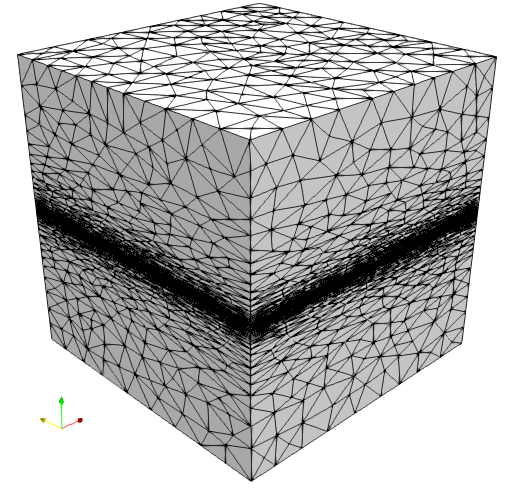
\includegraphics[width=\textwidth]{epic-ic-cube-linear.png}
\caption{EPIC-IC}
\end{subfigure}
\begin{subfigure}{.24\textwidth}
\centering
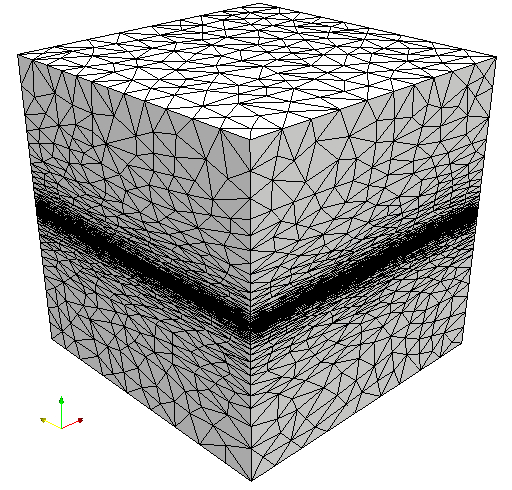
\includegraphics[width=\textwidth]{epic-ics-cube-linear.png}
\caption{EPIC-ICS}
\end{subfigure}
\begin{subfigure}{.24\textwidth}
\centering
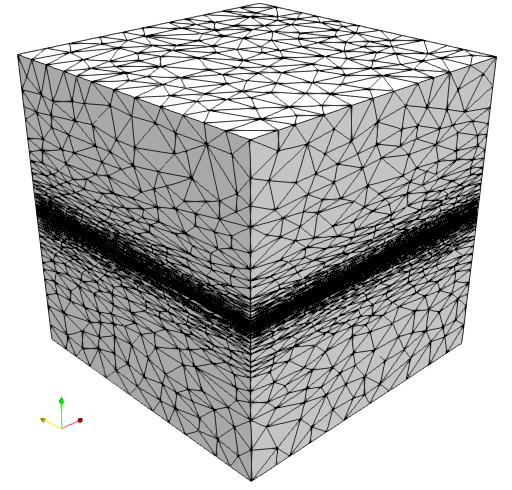
\includegraphics[width=\textwidth]{epic-icsm-cube-linear.png}
\caption{EPIC-ICSM}
\end{subfigure}
\begin{subfigure}{.24\textwidth}
\centering
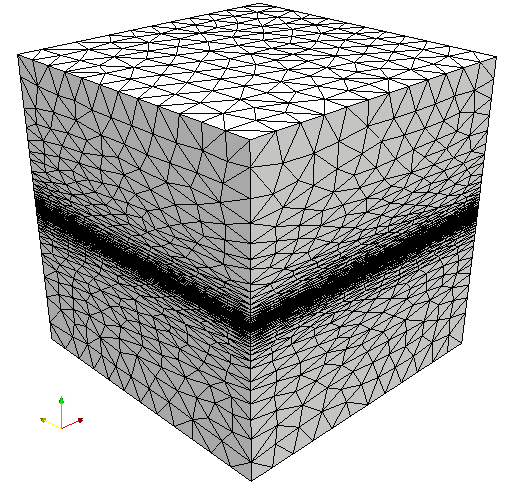
\includegraphics[width=\textwidth]{fefloa-cube-linear.png}
\caption{feflo.a}
\end{subfigure}
\begin{subfigure}{.24\textwidth}
\centering
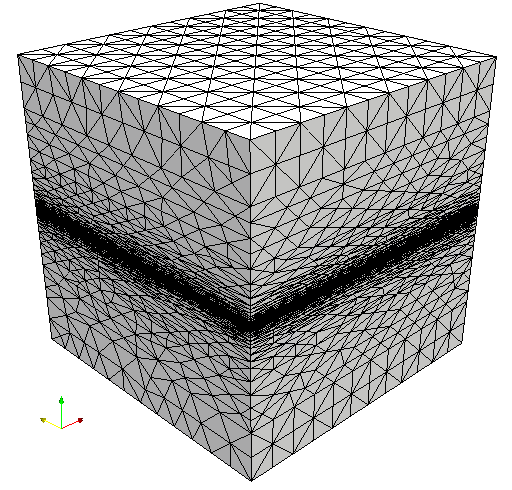
\includegraphics[width=\textwidth]{omega_h-cube-linear.png}
\caption{Omega\_h}
\end{subfigure}
\begin{subfigure}{.24\textwidth}
\centering
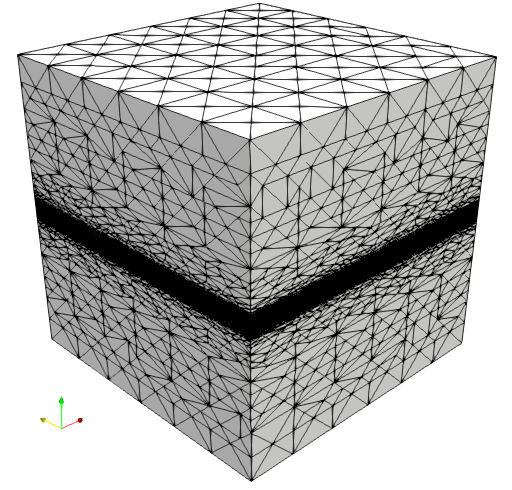
\includegraphics[width=\textwidth]{refine-one-cube-linear.png}
\caption{refine/one}
\end{subfigure}
\begin{subfigure}{.24\textwidth}
\centering
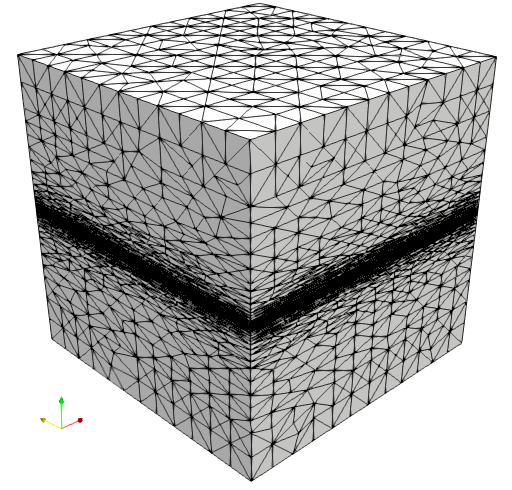
\includegraphics[width=\textwidth]{refine-two-cube-linear.png}
\caption{refine/two}
\end{subfigure}
\begin{subfigure}{.24\textwidth}
\centering
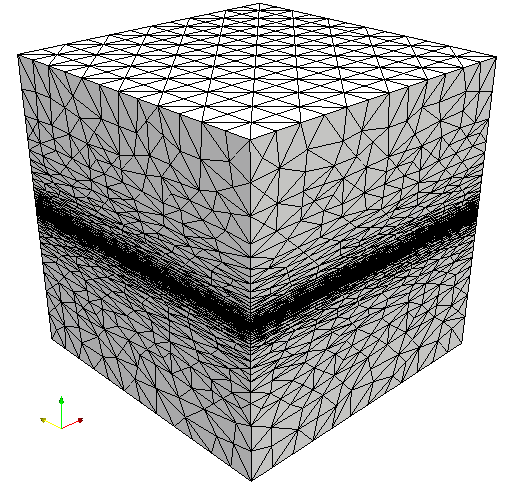
\includegraphics[width=\textwidth]{pragmatic-cube-linear.png}
\caption{Pragmatic}
\end{subfigure}
\caption{Meshes for the linear cube metric}
\label{fig:cube-linear-meshes}
\end{figure}

Table \ref{tab:cube-linear-stats} presents the statistics
for the satisfaction criteria that each code
produced with the linear metric input over the cube domain.
In the EPIC family, we see a clear improvement in minimum
quality and edge length range as operators are added
going from EPIC-IC to EPIC-ICS and EPIC-ICSM.
The high maximum length measures for EPIC are likely due
to the fact that it does not use Equations \ref{eq:length}
and \ref{eq:endpoint_lengths} to measure length
internally~\cite{park-loseille-krakos-michal-adapt-decomposition}.
Omega\_h, feflo.a, and refine/one
all achieve the same maximum length of 1.80, although
feflo.a and Omega\_h have higher qualities
and minimum lengths.
EPIC-IC, EPIC-ICS, and Omega\_h all get roughly
the same element count (50K), while EPIC-ICSM and feflo.a
get slightly better element counts (45K).
This is likely due to their use of smoothing (mesh motion),
which allows more fine tuning than topology modifications alone.
The feflo.a statistics are the best in terms of minimum
quality,
minimum length, and element count.

\begin{table}
\caption{Criteria statistics for linear cube metric}
\label{tab:cube-linear-stats}
\begin{tabular}{lrrrr}
Code & Min. Quality & Min. Length & Max. Length & \#Elements\\
EPIC-IC     & $0.10$&       $0.15$&       $3.48$&   $ 50860$\\
EPIC-ICS    & $0.25$&       $0.32$&       $3.05$&   $ 49262$\\
EPIC-ICSM   & $0.36$&       $0.39$&       $2.44$&   $ 45892$\\
feflo.a     & $0.49$&       $0.45$&       $1.80$&   $ 45158$\\
Omega\_h    & $0.30$&       $0.21$&       $1.80$&   $ 51666$\\
refine/one  & $0.06$&       $0.03$&       $1.80$&   $112543$\\
refine/two  & $0.05$&       $0.29$&       $1.67$&   $ 51587$\\
Pragmatic   & $0.46$&       $0.34$&       $1.67$&   $ 49332$\\
\end{tabular}
\end{table}

Figure \ref{fig:cube-linear-lengths} shows a more in-depth look
at the edge length distributions for the linear cube metric
via histograms.
Once again we see a distinction between codes with and without
smoothing, with flatter length profiles
for EPIC-IC, EPIC-ICS, and Omega\_h showing two distinct local maxima.
This is likely due to the use of upper and lower thresholds
to choose when to refine and coarsen edges.
A refinement can be viewed as removing an edge from a high
histogram bin and adding several edges to lower bins,
accumulating edges in bins just below the threshold.
Since the thresholds are typically spaced a factor of two apart,
we see the two accumulations of edges.
EPIC-ICSM and feflo.a show a much smoother, bell-curve-like distribution
with a single maximum.
Recall from Table \ref{tab:cube-linear-stats} that refine/one produces
twice as many elements as the other codes, and the explanation for this can be
found in Figure \ref{fig:cube-linear-lengths-refine-one}:
it produces many short edges that other codes coarsen.
\begin{figure}
\begin{subfigure}{.16\textwidth}
\centering
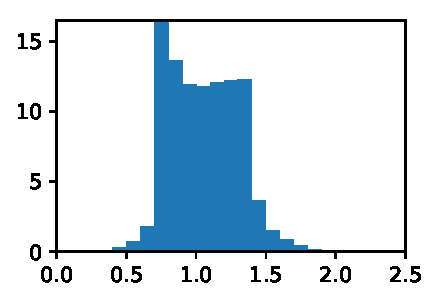
\includegraphics[width=\textwidth]{epic-ic-cube-linear-length.pdf}
\caption{EPIC-IC}
\end{subfigure}
\begin{subfigure}{.16\textwidth}
\centering
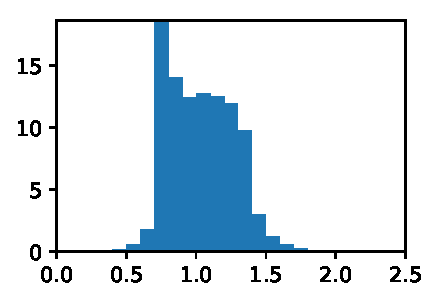
\includegraphics[width=\textwidth]{epic-ics-cube-linear-length.pdf}
\caption{EPIC-ICS}
\end{subfigure}
\begin{subfigure}{.16\textwidth}
\centering
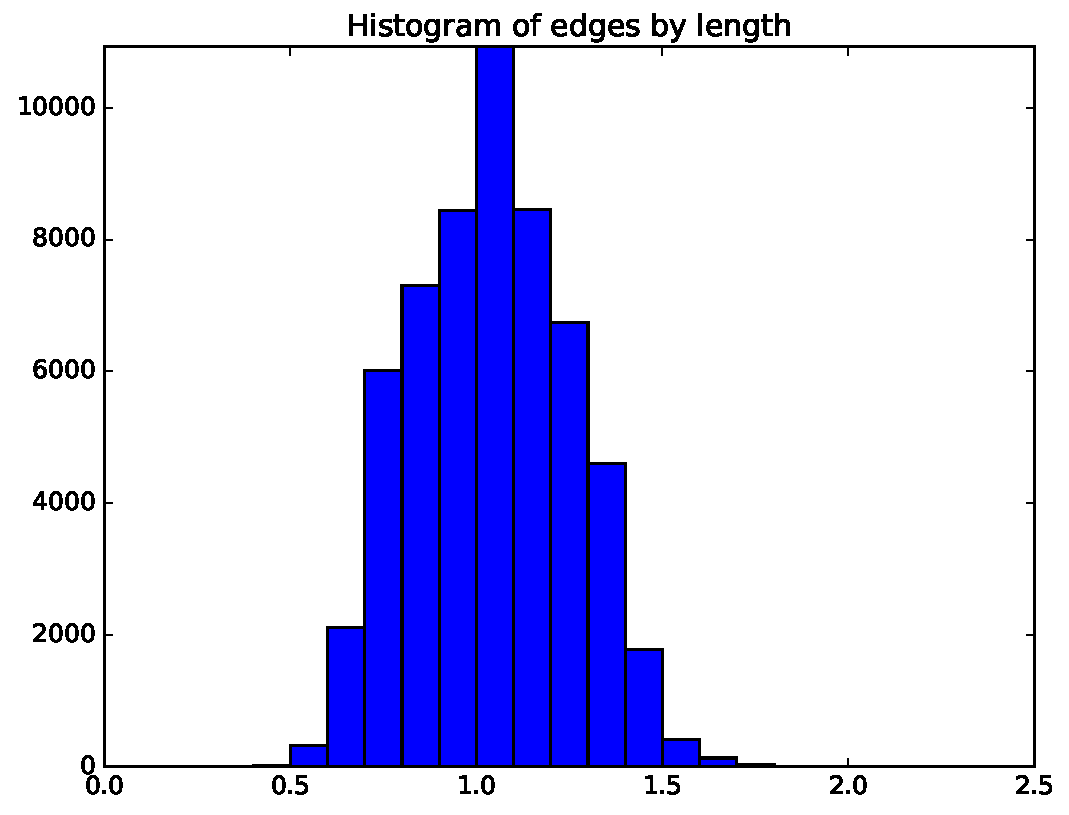
\includegraphics[width=\textwidth]{epic-icsm-cube-linear-length.pdf}
\caption{EPIC-ICSM}
\end{subfigure}
\begin{subfigure}{.16\textwidth}
\centering
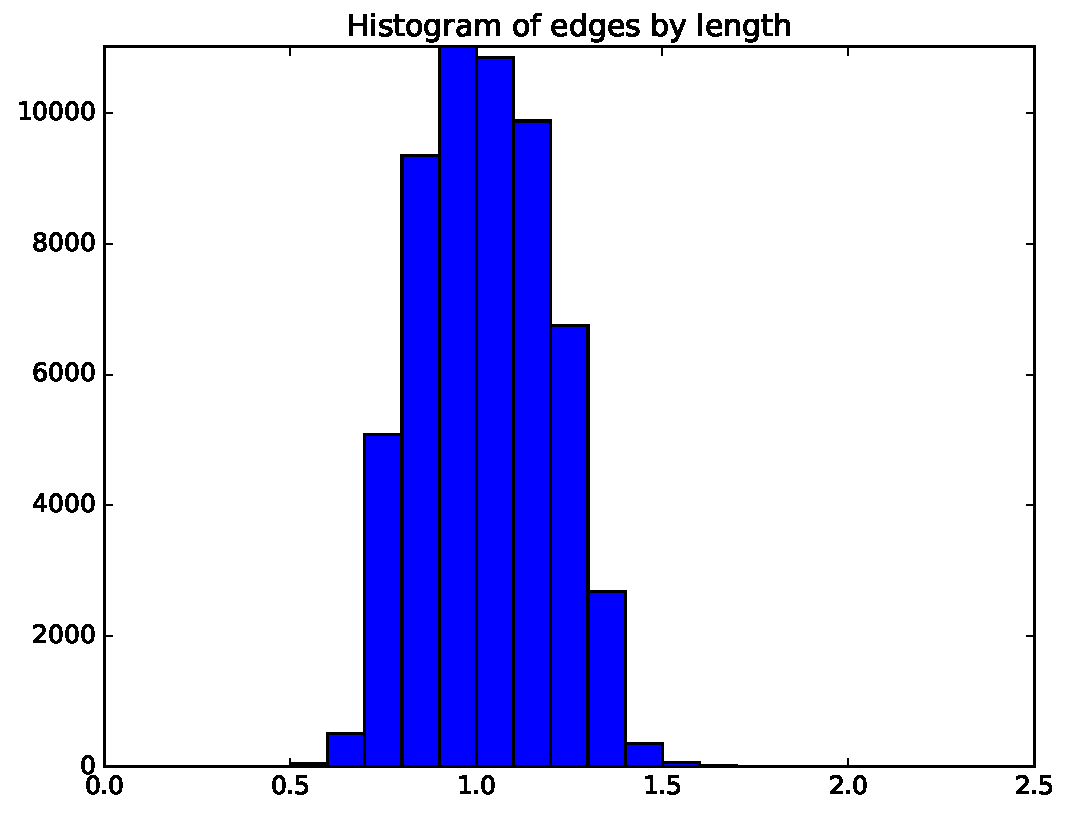
\includegraphics[width=\textwidth]{fefloa-cube-linear-length.pdf}
\caption{feflo.a}
\end{subfigure}
\begin{subfigure}{.16\textwidth}
\centering
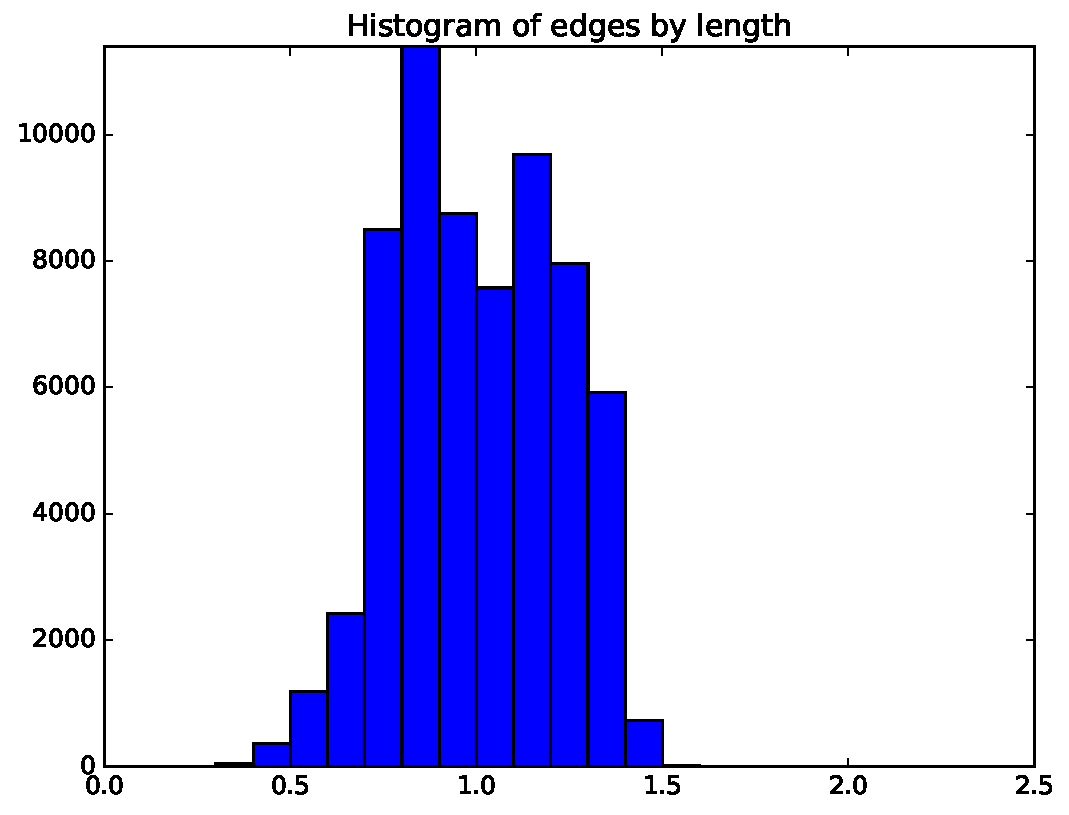
\includegraphics[width=\textwidth]{omega_h-cube-linear-length.pdf}
\caption{Omega\_h}
\end{subfigure}
\begin{subfigure}{.16\textwidth}
\centering
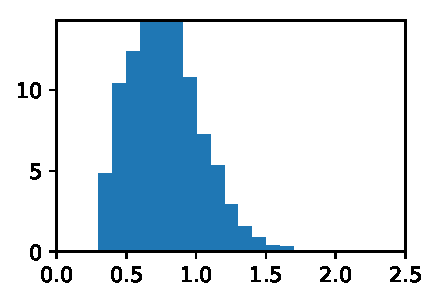
\includegraphics[width=\textwidth]{refine-one-cube-linear-length.pdf}
\caption{refine/one}
\label{fig:cube-linear-lengths-refine-one}
\end{subfigure}
\begin{subfigure}{.16\textwidth}
\centering
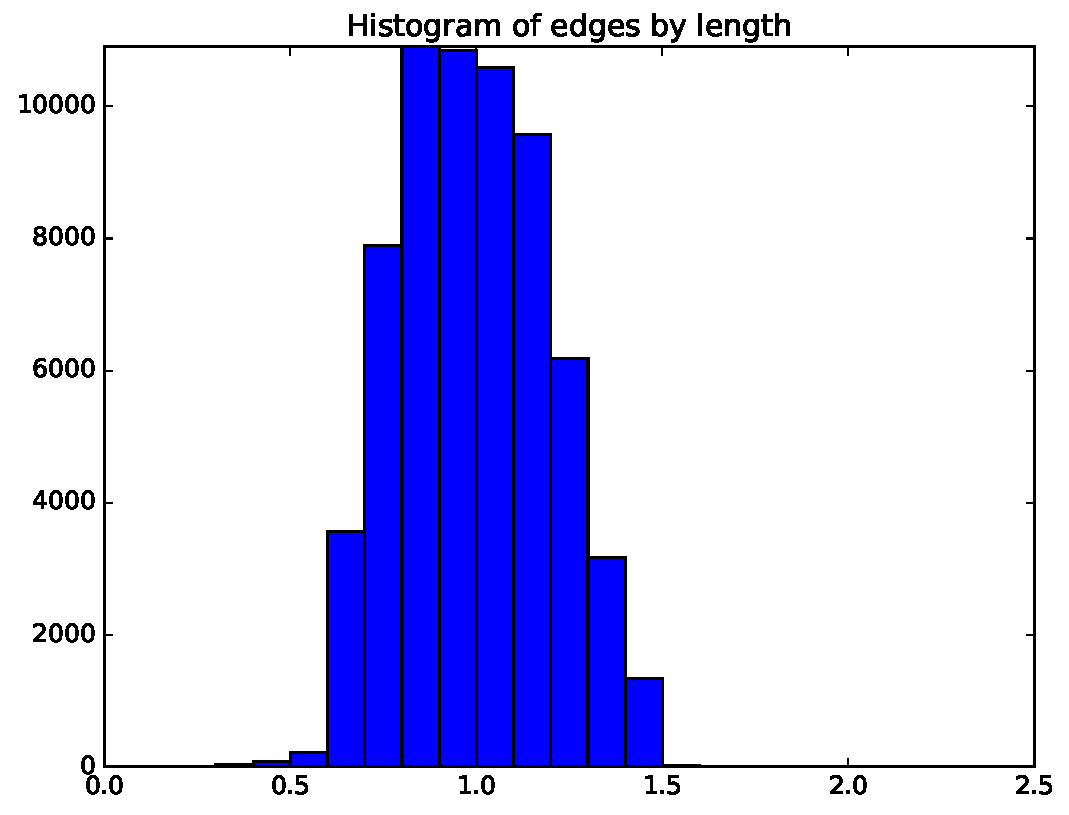
\includegraphics[width=\textwidth]{refine-two-cube-linear-length.pdf}
\caption{refine/two}
\end{subfigure}
\begin{subfigure}{.16\textwidth}
\centering
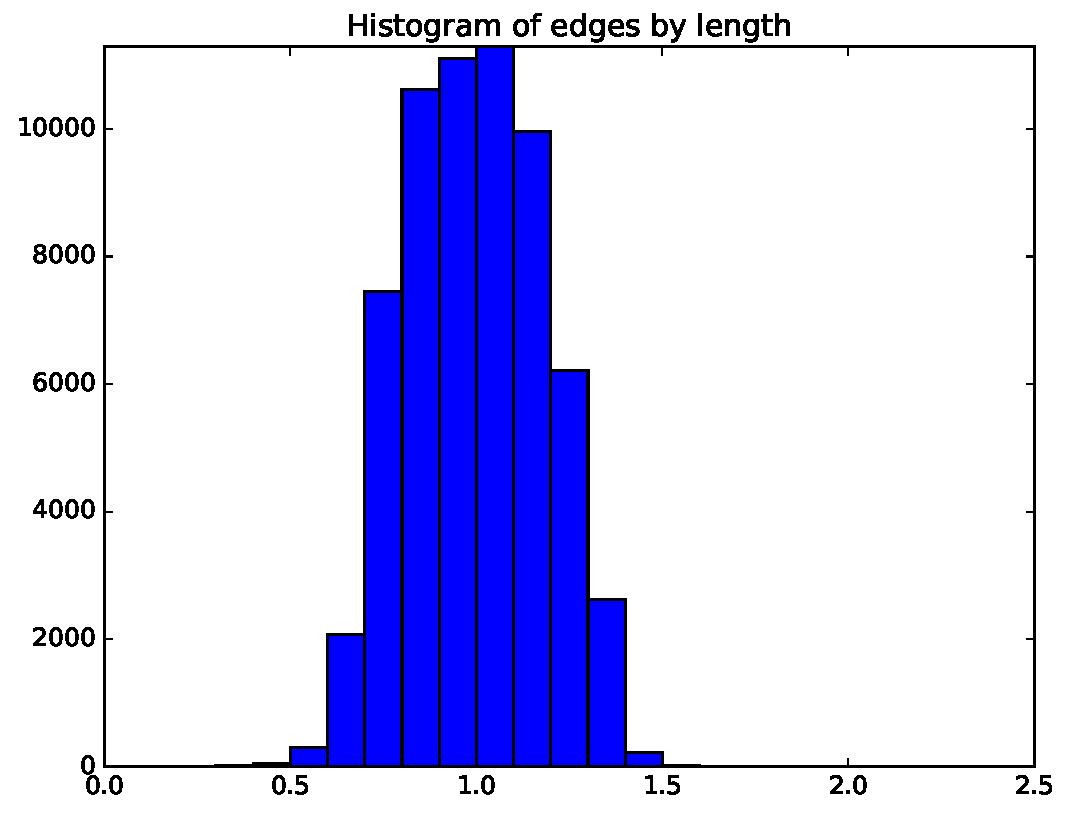
\includegraphics[width=\textwidth]{pragmatic-cube-linear-length.pdf}
\caption{Pragmatic}
\end{subfigure}
\caption{Length histograms for the linear cube metric}
\label{fig:cube-linear-lengths}
\end{figure}
The quality histograms for this case are omitted;
all codes showed similar distributions.

\subsection{Linear Cube-Cylinder Case}

There are three different metric cases with the Cube-Cylinder geometry,
which adds geometric curvature as a new difficulty.
\begin{figure}
\begin{subfigure}{.24\textwidth}
\centering
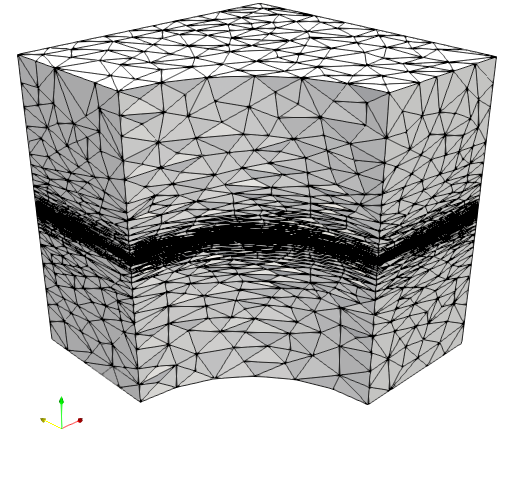
\includegraphics[width=\textwidth]{epic-ic-cube-cylinder-linear.png}
\caption{EPIC-IC}
\end{subfigure}
\begin{subfigure}{.24\textwidth}
\centering
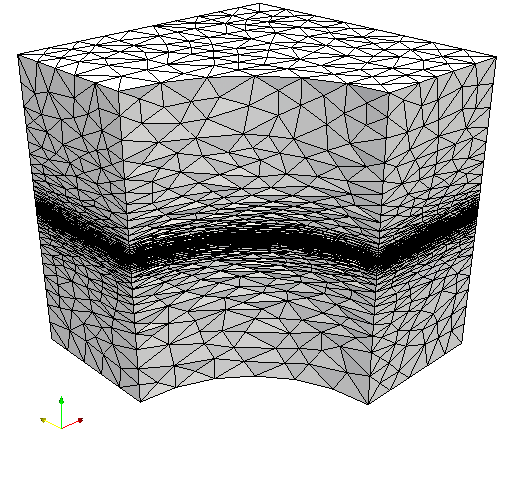
\includegraphics[width=\textwidth]{epic-ics-cube-cylinder-linear.png}
\caption{EPIC-ICS}
\end{subfigure}
\begin{subfigure}{.24\textwidth}
\centering
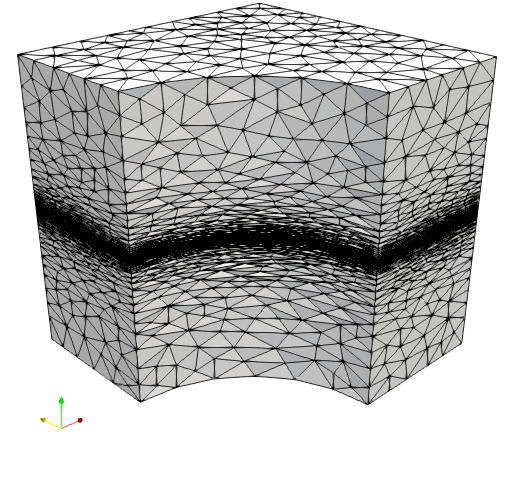
\includegraphics[width=\textwidth]{epic-icsm-cube-cylinder-linear.png}
\caption{EPIC-ICSM}
\end{subfigure}
\begin{subfigure}{.24\textwidth}
\centering
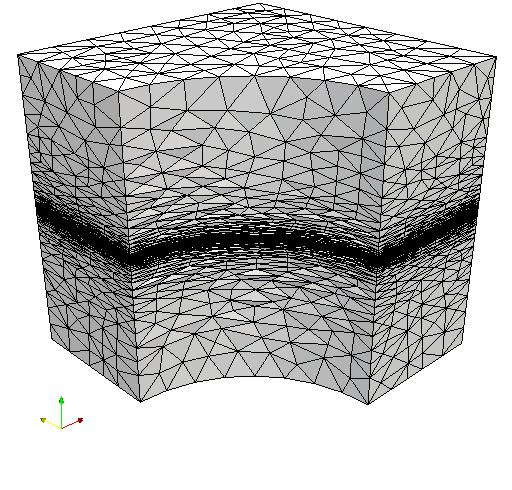
\includegraphics[width=\textwidth]{omega_h-cube-cylinder-linear.png}
\caption{Omega\_h}
\end{subfigure}
\begin{subfigure}{.24\textwidth}
\centering
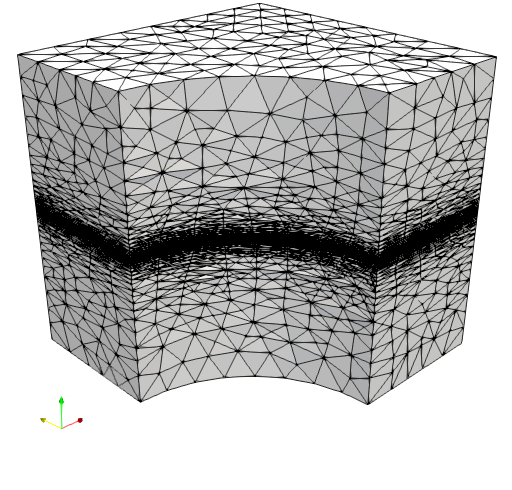
\includegraphics[width=\textwidth]{pragmatic-cube-cylinder-linear.png}
\caption{Pragmatic}
\end{subfigure}
\begin{subfigure}{.24\textwidth}
\centering
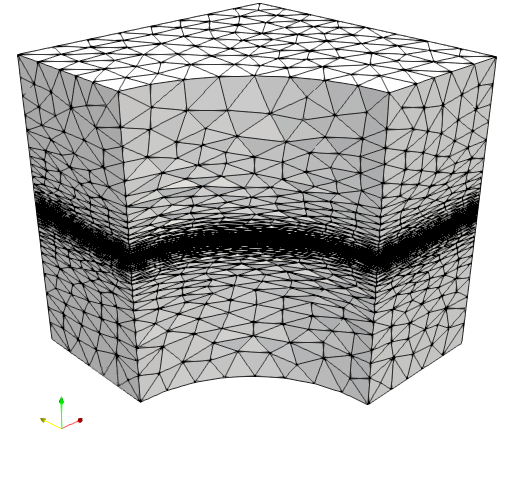
\includegraphics[width=\textwidth]{fefloa-cube-cylinder-linear.png}
\caption{feflo.a}
\end{subfigure}
\begin{subfigure}{.24\textwidth}
\centering
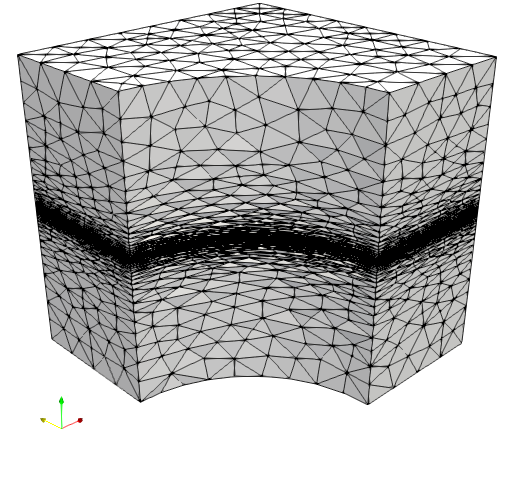
\includegraphics[width=\textwidth]{refine-two-cube-cylinder-linear.png}
\caption{refine/two}
\end{subfigure}
\caption{Meshes for the linear cube-cylinder metric}
\label{fig:cube-cylinder-linear-meshes}
\end{figure}
Table \ref{tab:cube-cylinder-linear-stats} shows minima
and maxima for the relevant criteria for each code.
The refine/one code is absent for cube-cylinder geometry cases,
because it has not implemented the EGADS API for curved geometry resolution.
On this geometry, we start to see EPIC-IC perform much
worse than other codes, with the longest edge being over
$50\times$ longer than desired, the shortest edge being
$100\times$ shorter than desired, and the minimum quality being
below the output precision of our measurement tools.
Fortunately, EPIC-ICS and EPIC-ICSM perform much better,
with edge length ranges similar to their cube results.
Omega\_h maintains its minimum quality at 30\%, and
has a decent edge length range, comparable to the EPIC codes.
While Pragmatic achieves a good maximum length bound,
its minimum length and quality are much smaller than they
were on the linear cube problem.

\begin{table}
\caption{Criteria statistics for linear cube-cylinder metric}
\label{tab:cube-cylinder-linear-stats}
\begin{tabular}{lrrrr}
Code & Min. Quality & Min. Length & Max. Length & \#Elements\\
EPIC-IC    &$<0.001$&       $0.01$&      $57.65$&    $32711$\\
EPIC-ICS   &  $0.16$&       $0.34$&      $ 2.83$&    $37481$\\
EPIC-ICSM  &  $0.19$&       $0.32$&      $ 3.26$&    $34236$\\
Omega\_h   &  $0.30$&       $0.29$&      $ 1.97$&    $40956$\\
Pragmatic  &  $0.01$&       $0.02$&      $ 2.06$&    $38668$\\
feflo.a    &  $0.04$&       $0.21$&      $ 2.55$&    $46291$\\
refine/two &  $0.04$&       $0.16$&      $ 1.73$&    $38668$\\
\end{tabular}
\end{table}

Figure \ref{fig:cube-cylinder-linear-lengths} presents edge lengths
as histograms.
Both EPIC-IC and EPIC-ICS show two local maxima.
At the extrema, EPIC-IC and Pragmatic both have noticeable
percentages of their edges in the very low range of $[0,0.25]$
while all the EPIC codes show a significant tail of edges
in the high range $[2.0,2.5]$.
\begin{figure}
\begin{subfigure}{.16\textwidth}
\centering
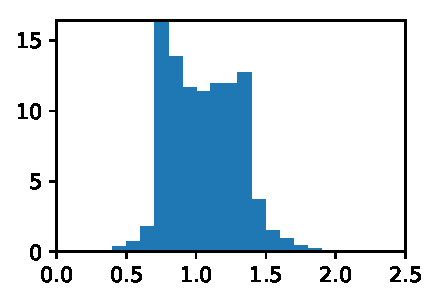
\includegraphics[width=\textwidth]{epic-ic-cube-cylinder-linear-length.pdf}
\caption{EPIC-IC}
\end{subfigure}
\begin{subfigure}{.16\textwidth}
\centering
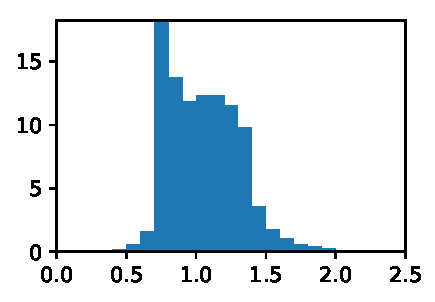
\includegraphics[width=\textwidth]{epic-ics-cube-cylinder-linear-length.pdf}
\caption{EPIC-ICS}
\end{subfigure}
\begin{subfigure}{.16\textwidth}
\centering
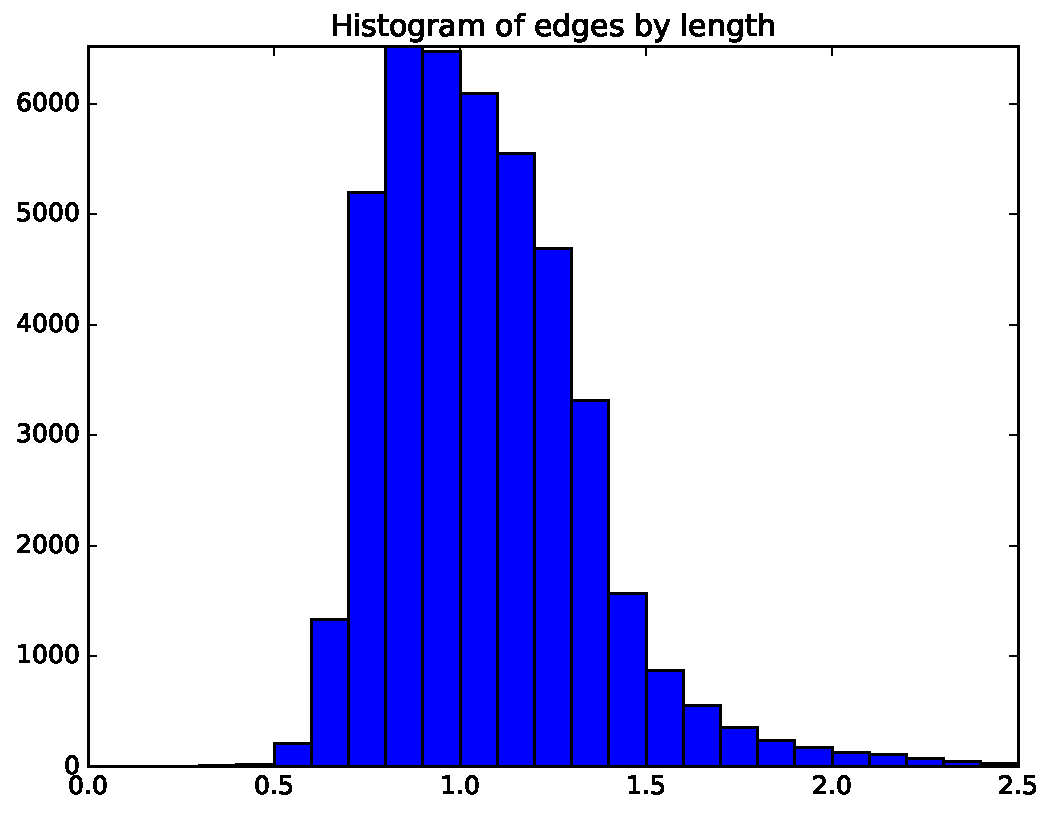
\includegraphics[width=\textwidth]{epic-icsm-cube-cylinder-linear-length.pdf}
\caption{EPIC-ICSM}
\end{subfigure}
\begin{subfigure}{.16\textwidth}
\centering
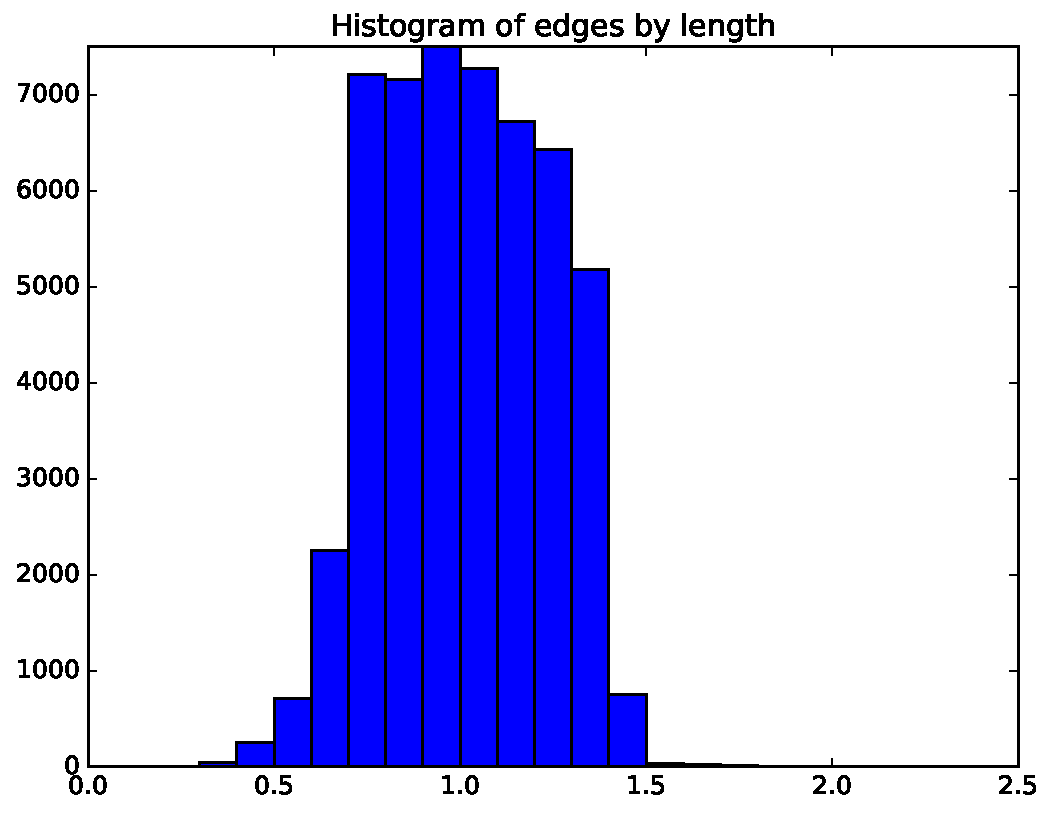
\includegraphics[width=\textwidth]{omega_h-cube-cylinder-linear-length.pdf}
\caption{Omega\_h}
\end{subfigure}
\begin{subfigure}{.16\textwidth}
\centering
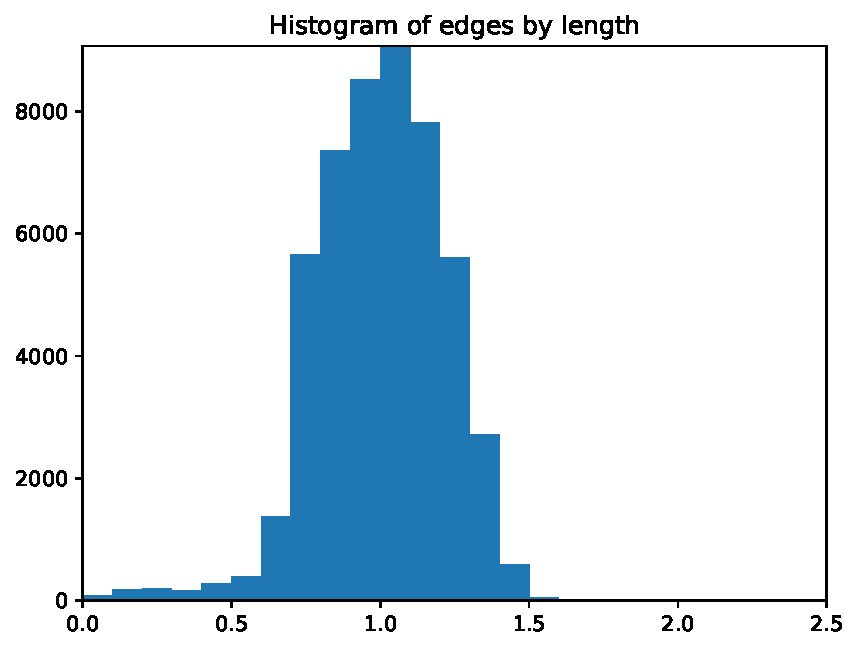
\includegraphics[width=\textwidth]{pragmatic-cube-cylinder-linear-length.pdf}
\caption{Pragmatic}
\end{subfigure}
\begin{subfigure}{.16\textwidth}
\centering
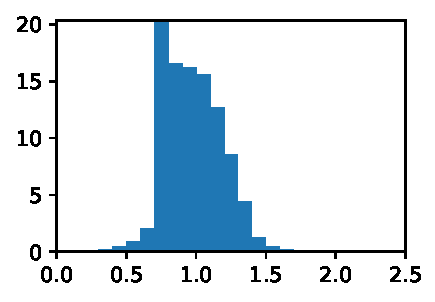
\includegraphics[width=\textwidth]{fefloa-cube-cylinder-linear-length.pdf}
\caption{feflo.a}
\end{subfigure}
\begin{subfigure}{.16\textwidth}
\centering
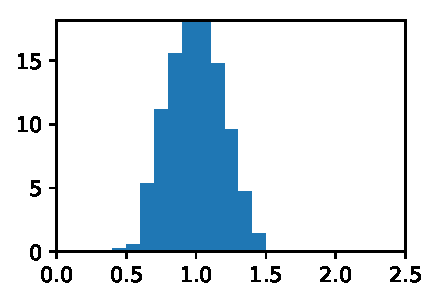
\includegraphics[width=\textwidth]{refine-two-cube-cylinder-linear-length.pdf}
\caption{refine/two}
\end{subfigure}
\caption{Length histograms for the linear cube-cylinder metric}
\label{fig:cube-cylinder-linear-lengths}
\end{figure}
The quality histograms for the linear cube-cylinder metric
are shown in Figure \ref{fig:cube-cylinder-linear-qualities}.
Here we see an interesting property of EPIC-IC on this geometry:
a spike of elements in the very low quality range $[0,0.1]$
which could not be corrected by its limited set of operators.
EPIC-ICS and EPIC-ICSM correct this spike, suggesting that
swapping is the key shape-correction operator.
The histograms of EPIC-ICS, EPIC-ICSM, and Omega\_h all look fairly
similar, which taper until no significant percentages can be
seen below 20\%, while Pragmatic has a tail of low-quality
elements that continue down to the lowest levels.
\begin{figure}
\begin{subfigure}{.16\textwidth}
\centering
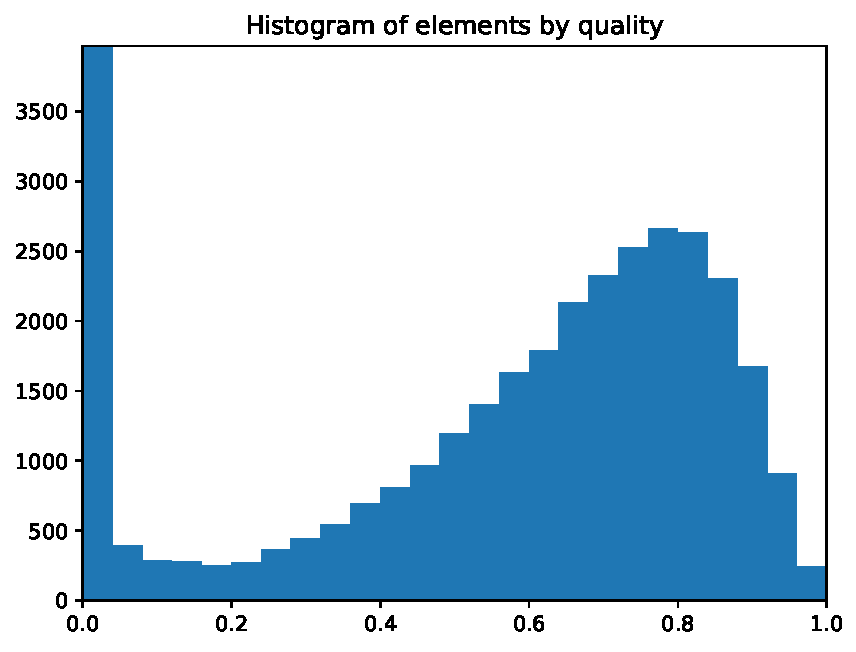
\includegraphics[width=\textwidth]{epic-ic-cube-cylinder-linear-quality.pdf}
\caption{EPIC-IC}
\end{subfigure}
\begin{subfigure}{.16\textwidth}
\centering
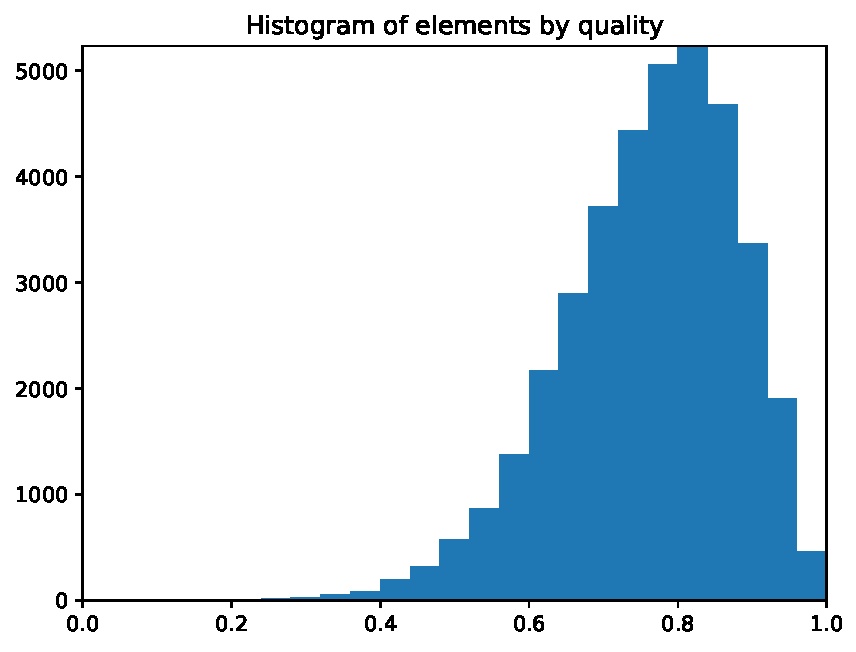
\includegraphics[width=\textwidth]{epic-ics-cube-cylinder-linear-quality.pdf}
\caption{EPIC-ICS}
\end{subfigure}
\begin{subfigure}{.16\textwidth}
\centering
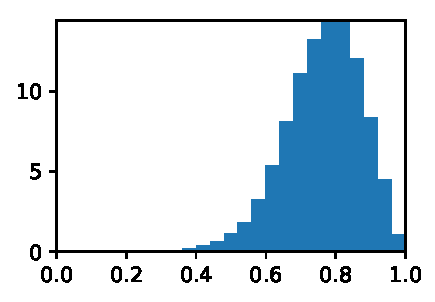
\includegraphics[width=\textwidth]{epic-icsm-cube-cylinder-linear-quality.pdf}
\caption{EPIC-ICSM}
\end{subfigure}
\begin{subfigure}{.16\textwidth}
\centering
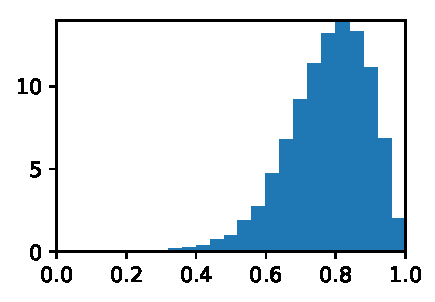
\includegraphics[width=\textwidth]{omega_h-cube-cylinder-linear-quality.pdf}
\caption{Omega\_h}
\end{subfigure}
\begin{subfigure}{.16\textwidth}
\centering
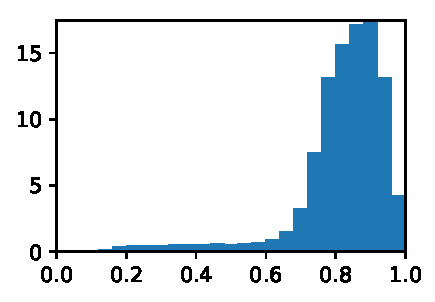
\includegraphics[width=\textwidth]{pragmatic-cube-cylinder-linear-quality.pdf}
\caption{Pragmatic}
\end{subfigure}
\begin{subfigure}{.16\textwidth}
\centering
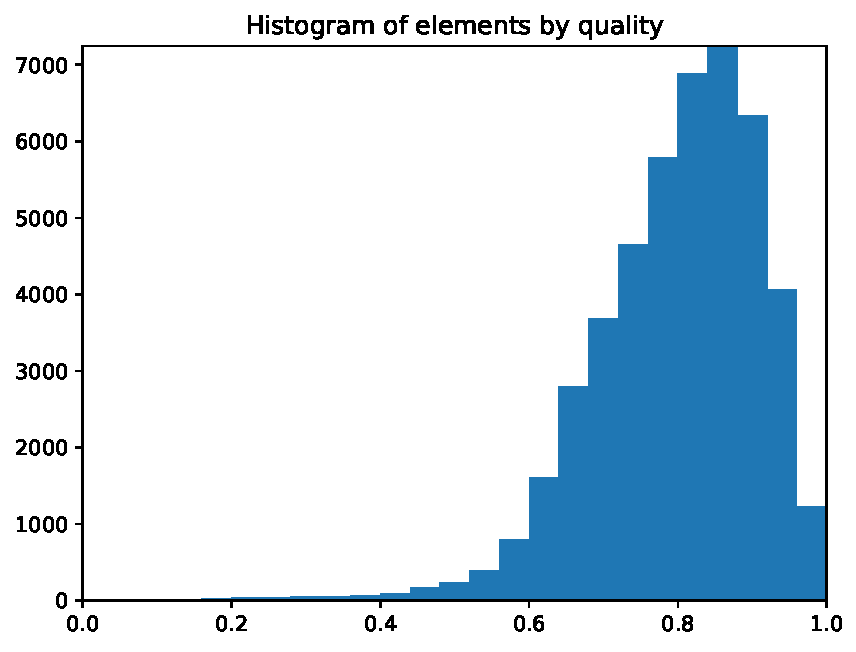
\includegraphics[width=\textwidth]{fefloa-cube-cylinder-linear-quality.pdf}
\caption{feflo.a}
\end{subfigure}
\begin{subfigure}{.16\textwidth}
\centering
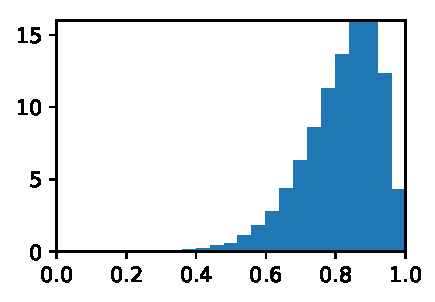
\includegraphics[width=\textwidth]{refine-two-cube-cylinder-linear-quality.pdf}
\caption{refine/two}
\end{subfigure}
\caption{Quality histograms for the linear cube-cylinder metric}
\label{fig:cube-cylinder-linear-qualities}
\end{figure}

\subsection{Polar-1 Cube-Cylinder Case}
\label{sec:cube-cylinder-polar-1}

Due to the curvature of the metric specification itself,
the main issue in satisfying this metric is high metric gradation.
As presented in Table \ref{tab:polar-1-stats}, all codes produced
a very low minimum quality.
\begin{figure}
\begin{subfigure}{.24\textwidth}
\centering
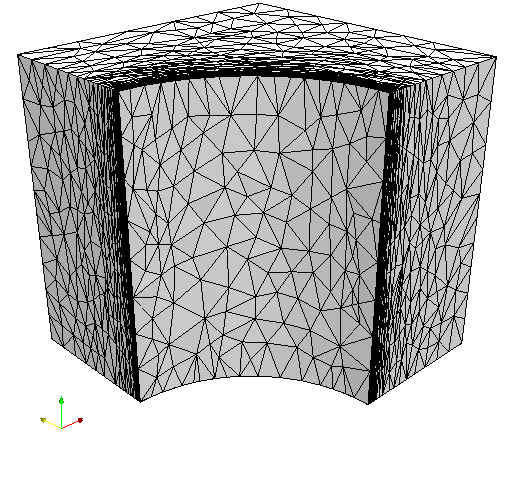
\includegraphics[width=\textwidth]{epic-ic-cube-cylinder-polar-1.png}
\caption{EPIC-IC}
\end{subfigure}
\begin{subfigure}{.24\textwidth}
\centering
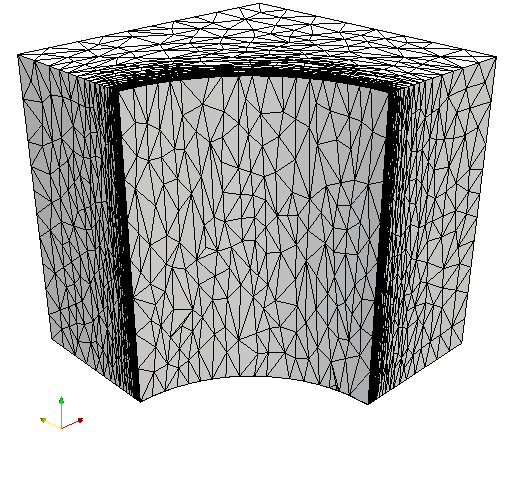
\includegraphics[width=\textwidth]{epic-ics-cube-cylinder-polar-1.png}
\caption{EPIC-ICS}
\end{subfigure}
\begin{subfigure}{.24\textwidth}
\centering
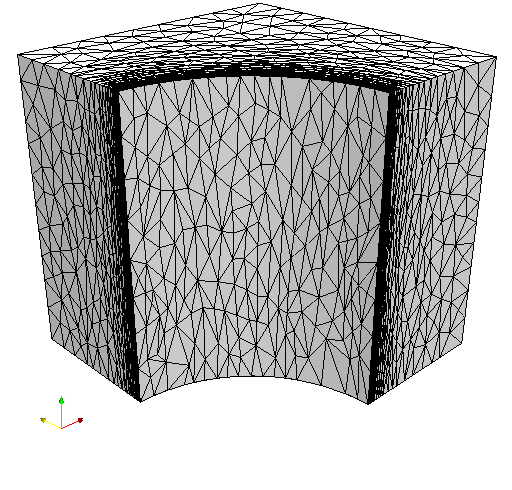
\includegraphics[width=\textwidth]{epic-icsm-cube-cylinder-polar-1.png}
\caption{EPIC-ICSM}
\end{subfigure}
\begin{subfigure}{.24\textwidth}
\centering
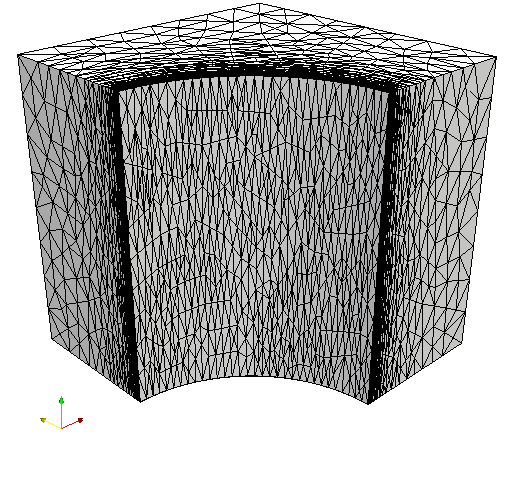
\includegraphics[width=\textwidth]{omega_h-cube-cylinder-polar-1.png}
\caption{Omega\_h}
\label{fig:omega_h-cube-cylinder-polar-1-mesh}
\end{subfigure}
\begin{subfigure}{.24\textwidth}
\centering
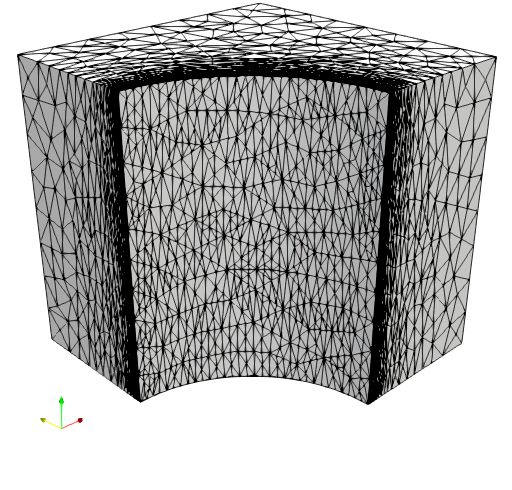
\includegraphics[width=\textwidth]{pragmatic-cube-cylinder-polar-1.png}
\caption{Pragmatic}
\end{subfigure}
\begin{subfigure}{.24\textwidth}
\centering
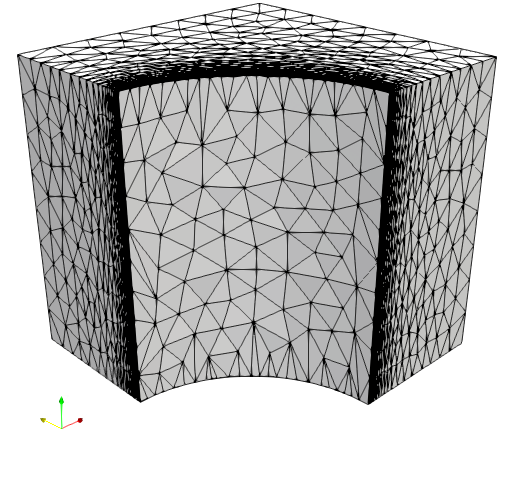
\includegraphics[width=\textwidth]{fefloa-cube-cylinder-polar-1.png}
\caption{feflo.a}
\label{fig:fefloa-cube-cylinder-polar-1-mesh}
\end{subfigure}
\caption{Meshes for the Polar-1 Cube-Cylinder metric}
\label{fig:cube-cylinder-polar-1-meshes}
\end{figure}
Omega\_h does not even converge if it cannot find a solution with
all elements above 30\% quality, so for this metric Omega\_h
pre-processed the metric using gradation control~\cite{Borouchaki-1998-gradation,alauzet-fead-2010-size-gradation-aniso}.
The resulting mesh is shown as the result in Figure~\ref{fig:omega_h-cube-cylinder-polar-1-mesh}.
This is what inspired the creation of the Polar-2 metric
(see Section \ref{sec:cube-cylinder-polar-2}),
which is an analytic equivalent of what gradation control did
to the metric.
In particular, it refines along the tangent direction
in order to reduce the rate of metric gradation due to curvature.
We still judge the resulting Omega\_h mesh by the original Polar-1
metric, hence it technically gets a minimum quality result of 14\% here.
EPIC-IC continues to show poor performance, while EPIC-ICS
and EPIC-ICSM show better performance.
EPIC-ICS and EPIC-ICSM have maximum lengths that are approximately
twice what they were in the linear cube-cylinder case in
Table \ref{tab:cube-cylinder-linear-stats}.
Pragmatic shows a good maximum length,
but has very small minimum lengths and qualities.
The curved surface mesh of feflo.a is clearly too coarse
(see Figure \ref{fig:fefloa-cube-cylinder-polar-1-mesh}),
likely due to not selecting the best option for handling
this highly graded metric.

\begin{table}
\caption{Criteria statistics for Polar-1 Cube-Cylinder metric}
\label{tab:polar-1-stats}
\begin{tabular}{lrrrr}
Code & Min. Quality & Min. Length & Max. Length & \#Elements\\
EPIC-IC    &$<0.001$&      $0.003$&      $67.64$&    $17338$\\
EPIC-ICS   &$  0.05$&      $ 0.13$&      $ 6.32$&    $21916$\\
EPIC-ICSM  &$  0.05$&      $ 0.20$&      $ 7.45$&    $20237$\\
Omega\_h   &$  0.14$&      $ 0.11$&      $ 1.71$&    $52235$\\
Pragmatic  &$  0.01$&      $ 0.02$&      $ 1.74$&    $33629$\\
feflo.a    &$  0.01$&      $ 0.18$&      $17.40$&    $35310$\\
\end{tabular}
\end{table}

Length histograms for the Polar-1 metric in Figure \ref{fig:cube-cylinder-polar-1-lengths}
show similar patterns for the EPIC codes, with the main difference being the
reduction of small edges as operators are added.
Omega\_h and Pragmatic show similar and better controlled distributions, consistent
with their maximum edge length results.
feflo.a still shows a good distribution, illustrating how histograms alone
don't capture important details, and justifying our inclusion of tables of extrema
and renderings.
\begin{figure}
\begin{subfigure}{.16\textwidth}
\centering
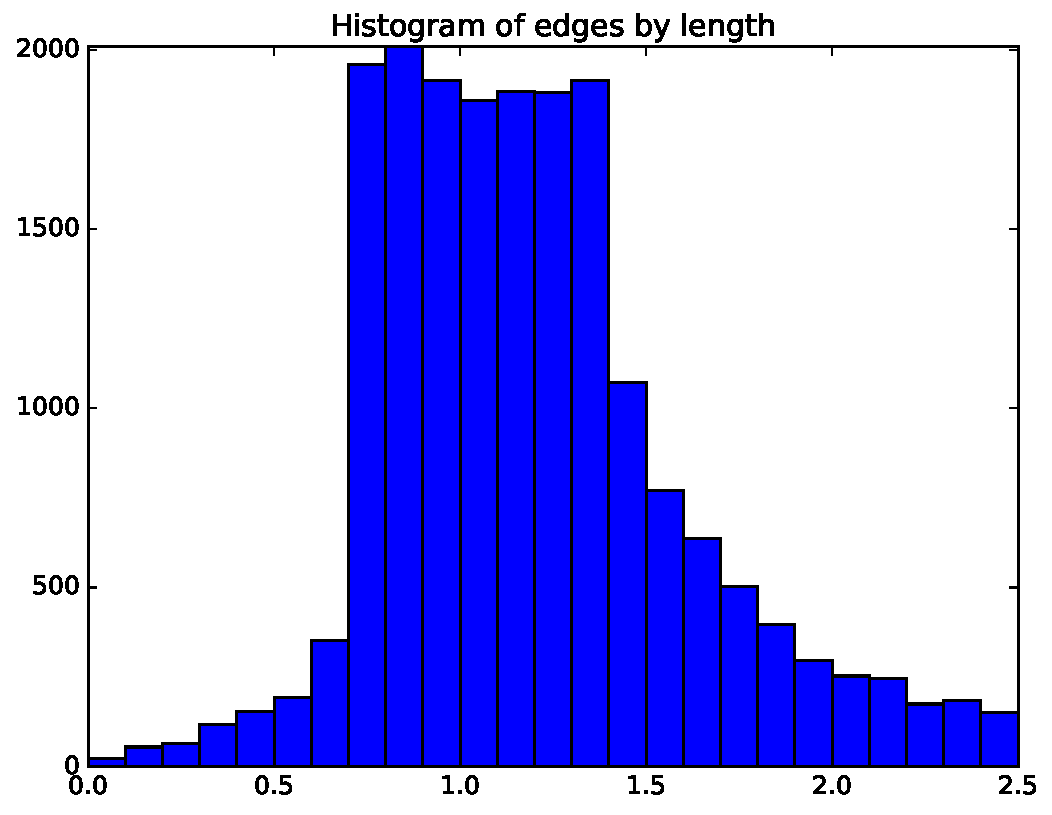
\includegraphics[width=\textwidth]{epic-ic-cube-cylinder-polar-1-length.pdf}
\caption{EPIC-IC}
\end{subfigure}
\begin{subfigure}{.16\textwidth}
\centering
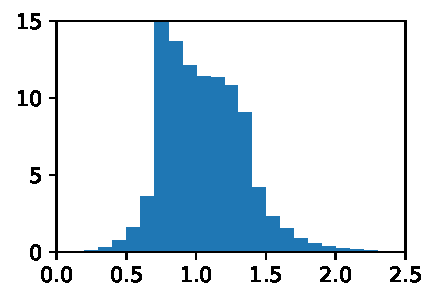
\includegraphics[width=\textwidth]{epic-ics-cube-cylinder-polar-1-length.pdf}
\caption{EPIC-ICS}
\end{subfigure}
\begin{subfigure}{.16\textwidth}
\centering
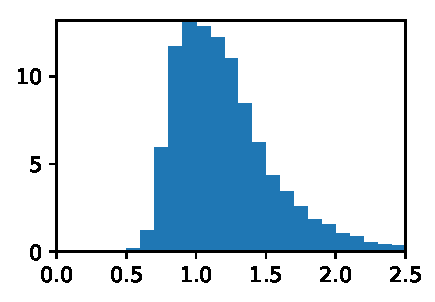
\includegraphics[width=\textwidth]{epic-icsm-cube-cylinder-polar-1-length.pdf}
\caption{EPIC-ICSM}
\end{subfigure}
\begin{subfigure}{.16\textwidth}
\centering
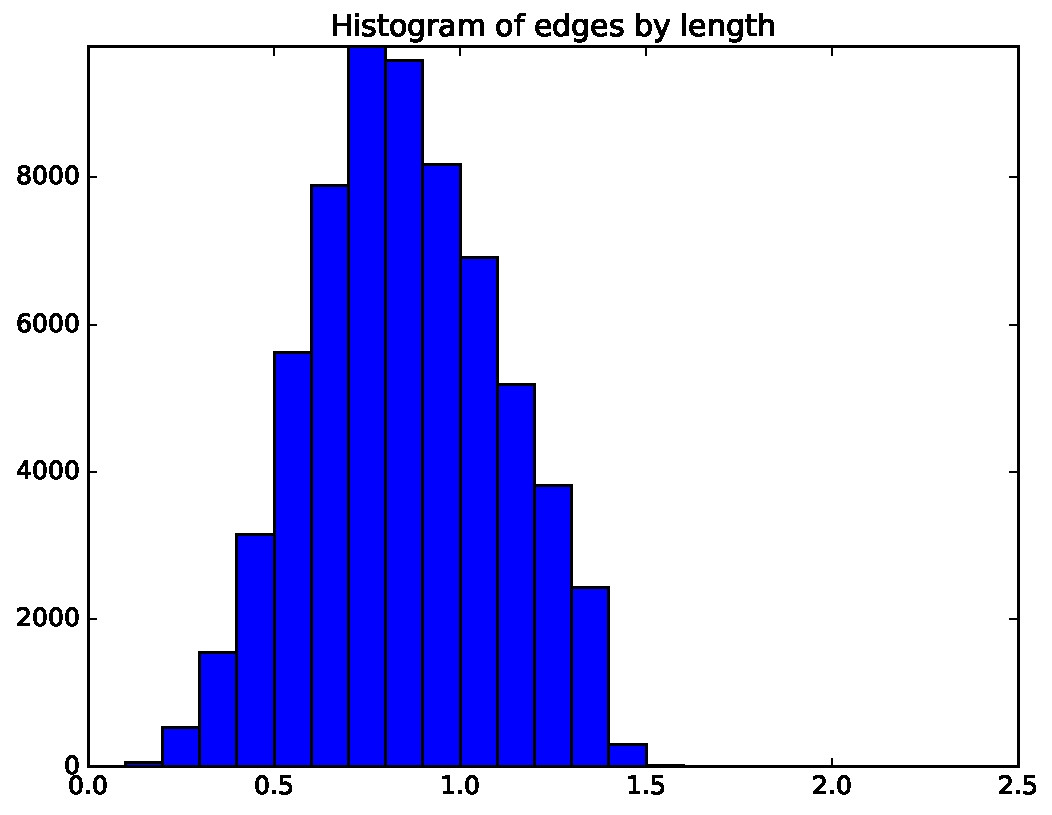
\includegraphics[width=\textwidth]{omega_h-cube-cylinder-polar-1-length.pdf}
\caption{Omega\_h}
\end{subfigure}
\begin{subfigure}{.16\textwidth}
\centering
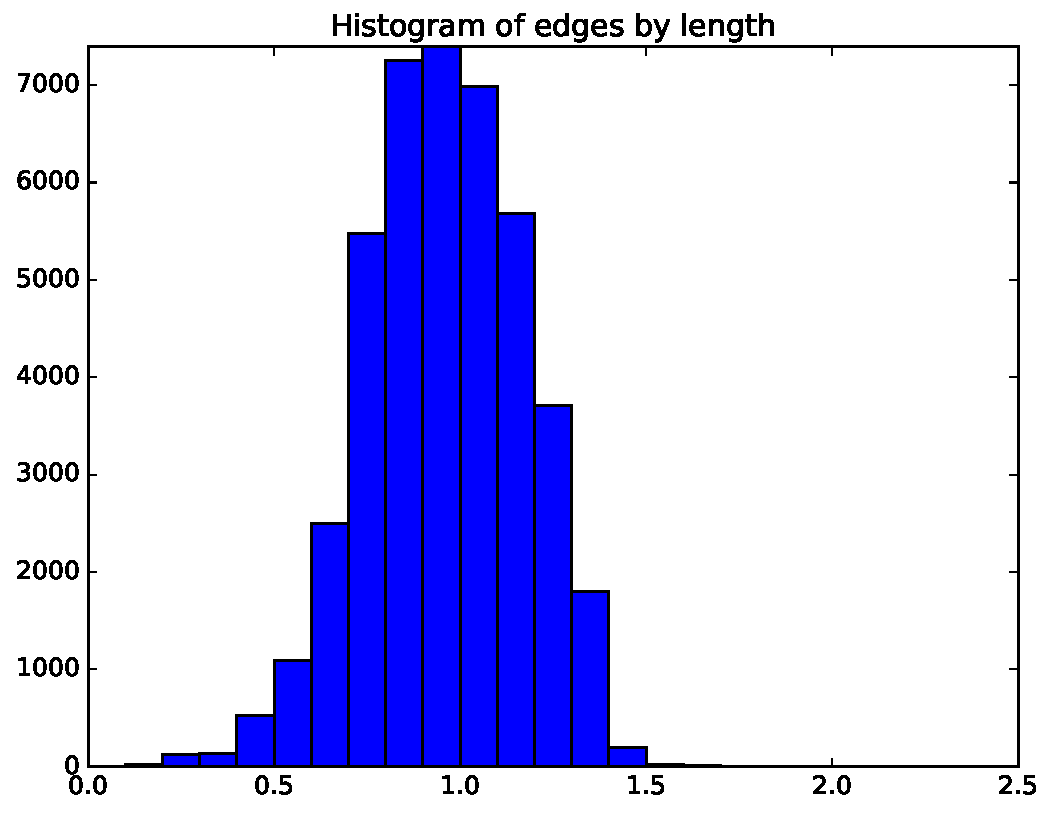
\includegraphics[width=\textwidth]{pragmatic-cube-cylinder-polar-1-length.pdf}
\caption{Pragmatic}
\end{subfigure}
\begin{subfigure}{.16\textwidth}
\centering
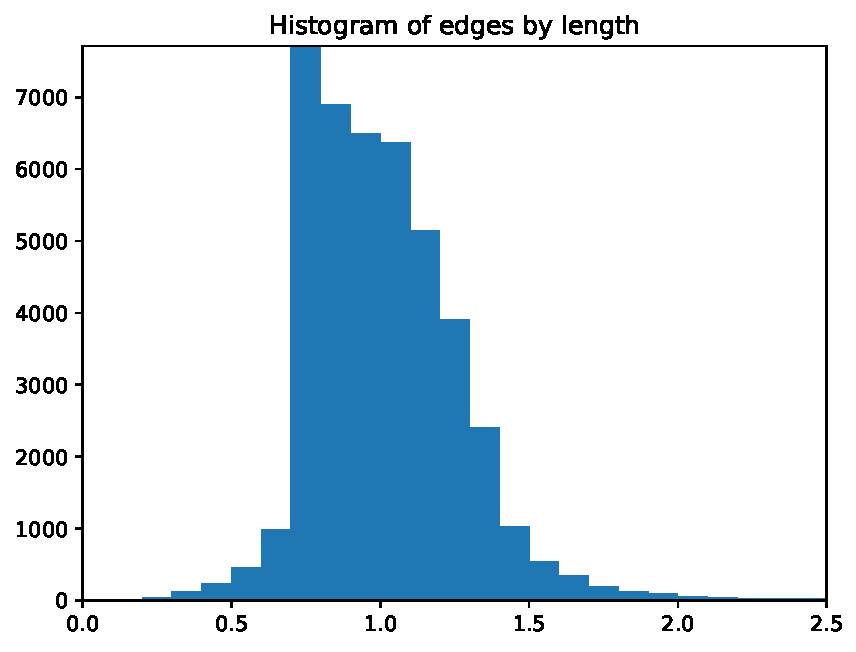
\includegraphics[width=\textwidth]{fefloa-cube-cylinder-polar-1-length.pdf}
\caption{feflo.a}
\end{subfigure}
\caption{Length histograms for the Polar-1 Cube-Cylinder metric}
\label{fig:cube-cylinder-polar-1-lengths}
\end{figure}
In the quality histograms (Figure \ref{fig:cube-cylinder-polar-1-qualities}),
EPIC-ICS, EPIC-ICSM, and Pragmatic have similar
profiles where frequency increases almost linearly with quality, but noticeable
amounts in very low range $[0,0.1]$.
Omega\_h has a different distribution, likely with a lower average quality,
but a much steeper and more controlled distribution in the low range.
\begin{figure}
\begin{subfigure}{.16\textwidth}
\centering
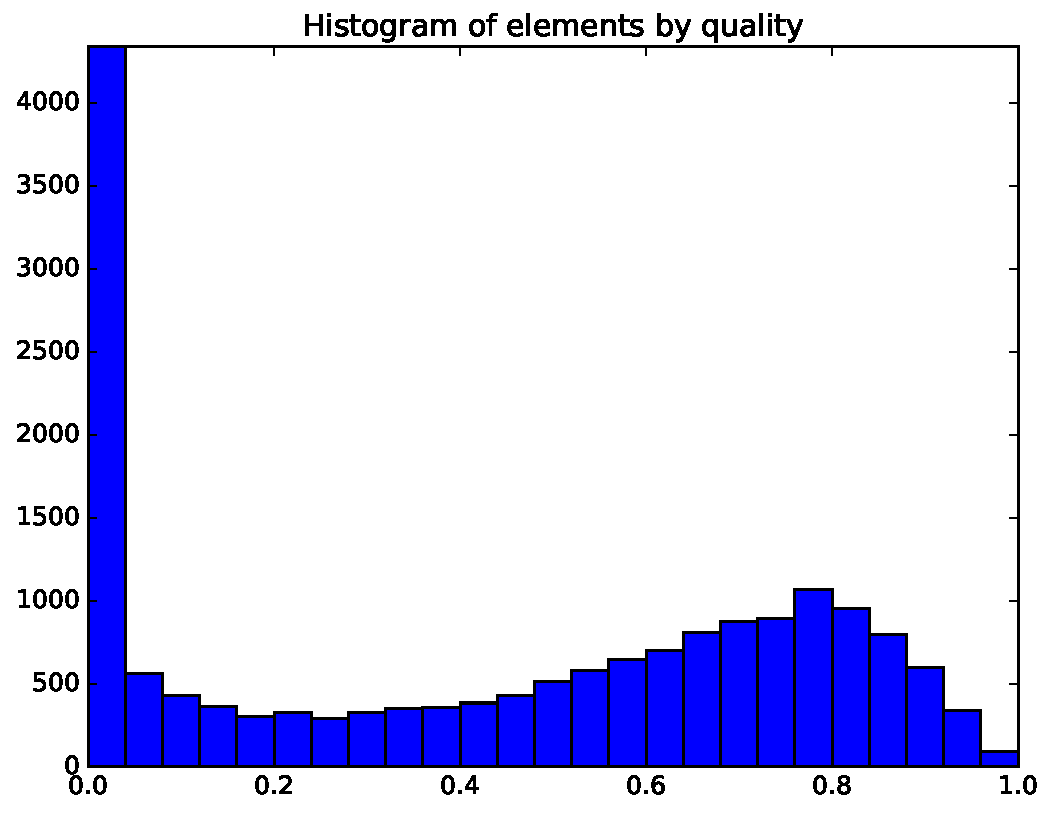
\includegraphics[width=\textwidth]{epic-ic-cube-cylinder-polar-1-quality.pdf}
\caption{EPIC-IC}
\end{subfigure}
\begin{subfigure}{.16\textwidth}
\centering
\includegraphics[width=\textwidth]{epic-ics-cube-cylinder-polar-1-quality.pdf}
\caption{EPIC-ICS}
\end{subfigure}
\begin{subfigure}{.16\textwidth}
\centering
\includegraphics[width=\textwidth]{epic-icsm-cube-cylinder-polar-1-quality.pdf}
\caption{EPIC-ICSM}
\end{subfigure}
\begin{subfigure}{.16\textwidth}
\centering
\includegraphics[width=\textwidth]{omega_h-cube-cylinder-polar-1-quality.pdf}
\caption{Omega\_h}
\label{fig:omega_h-cube-cylinder-polar-1-quality}
\end{subfigure}
\begin{subfigure}{.16\textwidth}
\centering
\includegraphics[width=\textwidth]{pragmatic-cube-cylinder-polar-1-quality.pdf}
\caption{Pragmatic}
\end{subfigure}
\begin{subfigure}{.16\textwidth}
\centering
\includegraphics[width=\textwidth]{fefloa-cube-cylinder-polar-1-quality.pdf}
\caption{feflo.a}
\end{subfigure}
\caption{Quality histograms for the Polar-1 Cube-Cylinder metric}
\label{fig:cube-cylinder-polar-1-qualities}
\end{figure}

\subsection{Polar-2 Cube-Cylinder Case}
\label{sec:cube-cylinder-polar-2}

The modification defining the Polar-2 metric specifically targets
a reduced gradation rate, and Table \ref{tab:polar-2-stats}
shows that the minimum qualities improved significantly for all
codes compared to Table \ref{tab:polar-1-stats} for Polar-1, suggesting a
connection between metric gradation rate and the best attainable
element quality.
Note also that EPIC-ICS and EPIC-ICSM have attained maximum lengths
on par with their usual best in the linear cases, suggesting that
gradation rate also has an effect on satisfiability of the metric
as measured by the length criteria.
Omega\_h is able to attain its threshold quality of 30\%, the best in the group.
Finally, note that if one compares the renderings
in Figure \ref{fig:cube-cylinder-polar-1-meshes} to those in
Figure \ref{fig:cube-cylinder-polar-2-meshes}, then EPIC-ICS,
EPIC-ICSM, and feflo.a are now much more in agreement with
Omega\_h and Pragmatic.

\begin{figure}
\begin{subfigure}{.24\textwidth}
\centering
\includegraphics[width=\textwidth]{epic-ic-cube-cylinder-polar-2.png}
\caption{EPIC-IC}
\end{subfigure}
\begin{subfigure}{.24\textwidth}
\centering
\includegraphics[width=\textwidth]{epic-ics-cube-cylinder-polar-2.png}
\caption{EPIC-ICS}
\end{subfigure}
\begin{subfigure}{.24\textwidth}
\centering
\includegraphics[width=\textwidth]{epic-icsm-cube-cylinder-polar-2.png}
\caption{EPIC-ICSM}
\end{subfigure}
\begin{subfigure}{.24\textwidth}
\centering
\includegraphics[width=\textwidth]{omega_h-cube-cylinder-polar-2.png}
\caption{Omega\_h}
\end{subfigure}
\begin{subfigure}{.24\textwidth}
\centering
\includegraphics[width=\textwidth]{pragmatic-cube-cylinder-polar-2.png}
\caption{Pragmatic}
\end{subfigure}
\begin{subfigure}{.24\textwidth}
\centering
\includegraphics[width=\textwidth]{fefloa-cube-cylinder-polar-2.png}
\caption{feflo.a}
\end{subfigure}
\caption{Meshes for the Polar-2 cube-cylinder metric}
\label{fig:cube-cylinder-polar-2-meshes}
\end{figure}

\begin{table}
\caption{Criteria statistics for Polar-2 Cube-Cylinder metric}
\label{tab:polar-2-stats}
\begin{tabular}{lrrrr}
Code & Min. Quality & Min. Length & Max. Length & \#Elements\\
EPIC-IC    &$<0.001$&     $<0.001$&      $70.53$&    $21664$\\
EPIC-ICS   &$  0.15$&     $  0.30$&      $ 3.01$&    $36538$\\
EPIC-ICSM  &$  0.19$&     $  0.45$&      $ 3.04$&    $33417$\\
Omega\_h   &$  0.30$&     $  0.24$&      $ 1.81$&    $49151$\\
Pragmatic  &$  0.05$&     $  0.12$&      $ 1.73$&    $47203$\\
feflo.a    &$  0.06$&     $  0.18$&      $ 2.65$&    $53117$\\
\end{tabular}
\end{table}

The length histograms for the Polar-2 metric were largely the
same as for the Polar-1 metric
(Figure \ref{fig:cube-cylinder-polar-1-lengths}),
and we omit them for brevity.
The quality histograms, on the other hand, show very significant differences
between the Polar-1 metric in Figure \ref{fig:cube-cylinder-polar-1-qualities}
and the Polar-2 metric in Figure \ref{fig:cube-cylinder-polar-2-qualities}.
All codes (except EPIC-IC) now show a good distribution of quality centered to the
far right with no noticeable percentages in the low range $[0,0.2]$.
Omega\_h also shows this nominal distribution, as opposed the strange distribution
it had in Figure \ref{fig:omega_h-cube-cylinder-polar-1-quality}.
This supports the idea that metric gradation has a significant effect not just
on minimum attainable quality but on the qualities of elements all throughout the mesh.

\begin{figure}
\begin{subfigure}{.16\textwidth}
\centering
\includegraphics[width=\textwidth]{epic-ic-cube-cylinder-polar-2-quality.pdf}
\caption{EPIC-IC}
\end{subfigure}
\begin{subfigure}{.16\textwidth}
\centering
\includegraphics[width=\textwidth]{epic-ics-cube-cylinder-polar-2-quality.pdf}
\caption{EPIC-ICS}
\end{subfigure}
\begin{subfigure}{.16\textwidth}
\centering
\includegraphics[width=\textwidth]{epic-icsm-cube-cylinder-polar-2-quality.pdf}
\caption{EPIC-ICSM}
\end{subfigure}
\begin{subfigure}{.16\textwidth}
\centering
\includegraphics[width=\textwidth]{omega_h-cube-cylinder-polar-2-quality.pdf}
\caption{Omega\_h}
\end{subfigure}
\begin{subfigure}{.16\textwidth}
\centering
\includegraphics[width=\textwidth]{pragmatic-cube-cylinder-polar-2-quality.pdf}
\caption{Pragmatic}
\end{subfigure}
\begin{subfigure}{.16\textwidth}
\centering
\includegraphics[width=\textwidth]{fefloa-cube-cylinder-polar-2-quality.pdf}
\caption{feflo.a}
\end{subfigure}
\caption{Quality histograms for the Polar-2 cube-cylinder metric}
\label{fig:cube-cylinder-polar-2-qualities}
\end{figure}


\section{Future Directions}

Unstructured mesh adaptation has proven to be a reliable tool
to predict complex phenomena
with complex geometries~\cite{alauzet-loseille-decade-aniso-adapt-cfd,%
  michal-unstruct-adapt-epic-dpw6}~for steady and unsteady flow regimes.
The adaptive process is an iterative procedure where  the mesh and
the solution are updated to reach {\it an optimal} mesh solution couple of a desired level of accuracy.
We decompose this process into:
(1) error estimation, (2) mesh generation, and (3) solution computation.
%One benefit of unstructured mesh adaptation is its ability to adapt to complex geometries as typically  found in aeronautic applications for instance:  landing gear, high lift configurations. Several
%algorithms to generate anisotropic meshes  with complex geometries exist.  We mention:  (i) edge-based, (iii) cavity-based or
% (iv) advancing-point-based.  For the flow solver, we consider second order turbulent flow solver.
%
However, the full benefit of adaptivity is then achieved only when (1), (2), and (3) are optimally combined.
This first set of benchmarks focus on analytic metric-conformity for a simple geometry.
We list the main issues that will be addressed by the next sets of test cases  for the verification and validation of mesh generation:

\emph{Surface mesh adaptation.\;}
Surface mesh adaptation becomes critical when an initial mesh is used as in the local re-meshing approach.
This is even more critical when a boundary layer or highly anisotropic areas  are present in the initial mesh and need to be modified.
Indeed, due to the presence of the volume mesh near the surface mesh, refining an element may lead to the creation
of a negative volume element.  
%The necessary level of discretization
%on the surface is currently never reached in the current best practice grids.
This high level of anisotropy has to be then correctly blended
with the  surface approximation estimate in order not to create numerical artifacts on the geometry.
The quality, level of anisotropy, robustness and CPU time need to be assessed  for the  algorithms described in this paper.
We intend to provide test cases  starting from more complex initial meshes and with a very high level of anisotropy
near the surface.
These challenging initial meshes and metrics assess the robustness of the surface mesh adaptation component with respect to the initial starting mesh
and the level of anisotropy.
%\begin{itemize}
%\item edge-based operators with standard optimizations (smoothing, face-edge swaps)
%\item point-frontal and cavity-based algorithms.
%\end{itemize}

\emph{CAD integration.\;}
For industrial applications, the use of CAD data is crucial as many quantities of interest
depends on the geometry. Providing high quality surface mesh becomes a mandatory feature.
We intend to define simple test cases featuring one typical CAD issue at a time:
missing topology,
CAD tolerance to edges larger than the required mesh size,
and highly skewed parameterization.

\emph{Adaptive boundary layer.\;}
The generation of a boundary layer mesh is generally designed for isotropic surface grids,
and is generated only once~\cite{pirzadeh-advancing-layer,loseille-lohner-imr21-robust-bl-gen}.
Consequently, the boundary layer is frozen while adapting
the outer part of the domain~\cite{park-carlson-turbulent-output-adapt-aiaa}.
However, this frozen boundary layer mesh strategy
is insufficient when the boundary layer
interacts when other anisotropic features.
The design and assessment of algorithms that are well suited to quickly generate boundary layer meshes
in the presence of anisotropic surface meshes is necessary.
Test cases will be designed with:
(i) an analytical boundary layer metric,
and (ii) a solution-based boundary layer metric. 

\emph{Parallel environment.\;}
Finally, the (potential) integration into an HPC environment~\cite{jansson-hoffman-jansson-siamjsc-2012-para-adapt-fe-cfd} of each previous mesh refinement techniques needs to be studied.
We intend to re-visit all the database test cases in a parallel environment.
In particular,
we can discuss the quality of the generated parallel grids with respect to the sequential one,
and also assess the performance advantage of the parallel mesh generation (for surface and volume).

In a more general setting, we then intend to extend progressively the number of test cases and results to more complex geometries and metrics
following the discussion of Park wt al.~\cite{park-unstruct-adapt-status-cfd2030}.
We will apply the same approach as in the preliminary study~\cite{park-loseille-krakos-michal-adapt-decomposition},
where only one component is modified (for instance, the error estimate) while the remaining
components are kept unchanged (e.g., flow solver, mesh generation algorithm).

\section{Conclusion}

These benchmark cases have revealed
a surprising number of useful insights both into the qualities of participating codes and the
nature of mesh adaptation in general.
The polar metrics illustrates how metric gradation can make the metric difficult to satisfy,
and how gradation control improves metric conformance across all the participating codes.
We see that the use of a different edge length criteria by EPIC tends to produce longer edges
and fewer elements compared to the other codes,
which is important to know when specifying metrics to a certain code.
The linear cube metric shows us that in certain cases using nodal repositioning as EPIC and feflo.a do can increase element quality
beyond what is feasible with topology modification alone,
while the cube-cylinder cases show that preventing low-quality modifications, as Omega\_h does, better
controls the worst element quality in the more difficult cases.

The Unstructured Grid Adaptation Working Group hopes
these and future benchmarks can serve as a common reference point for research in our field.
We invite others to apply the benchmark to their codes and
submit their results to the repository.
Ideas for improvements or additions to the benchmark cases are also welcome.

\bibliography{references}
\bibliographystyle{model1-num-names}

\end{document}
